\documentclass[letterpaper,10pt]{article}

% Soporte para los acentos.
\usepackage[utf8]{inputenc}
\usepackage[T1]{fontenc}    
% Idioma español.
\usepackage[spanish,mexico, es-tabla]{babel}
% Soporte de símbolos adicionales (matemáticas)
\usepackage{multirow}
\usepackage{amsmath}		
\usepackage{amssymb}		
\usepackage{amsthm}
\usepackage{amsfonts}
\usepackage{latexsym}
\usepackage{enumerate}
\usepackage{graphicx} %Para Insertar Imágenes
% Modificamos los márgenes del documento.
\usepackage[lmargin=2cm,rmargin=2cm,top=2cm,bottom=2cm]{geometry}
% Soporte para dibujar con Tikz.
\usepackage{tikz}
\usetikzlibrary{automata, positioning, arrows}

% Información para el título
\title{Autómatas y Lenguajes Formales\\ Tarea 3}
\author{Rodríguez Torres Víctor Fidel\\
Rubí Rojas Tania Michelle}
\date{06 de noviembre de 2018}

\begin{document}
    \maketitle
    
    \begin{enumerate}
    % Ejercicio 1.
        \item Para cada uno de los siguientes lenguajes da una descripción detallada de
        una máquina de Turing que los reconozca (puede ser una máquina de Turing
        sencilla, multicinta, o no-determinista pero la descripción debe ser detallada).
        \begin{itemize}
            
            % Lenguaje 1.
            \item $\{a^{n}b^{2n}$ $|$ $n \in \mathbb{N}\}$ \\ \\
            \textit{Solución:} La máquina de Turing que reconoce este lenguaje
            tiene el siguiente comportamiento
            \begin{figure}[ht]
               \centering
               \begin{tikzpicture}[->,>=stealth',shorten >=1pt,auto,node
                  distance=3.0cm, semithick]
                  
                  % Asignamos los estados del autómata.
                  \node[state,  initial] (q0) {$q_0$};
                  \node[state, right of=q0] (q1) {$q_1$};
                  \node[state, right of=q1] (q2) {$q_2$};
                  \node[state, below of=q2] (q3) {$q_3$};
                  \node[state, below  of=q0] (q4) {$q_4$};
                  \node[state, accepting, right of=q4] (q5) {$q_a$};
                  
                  % Dibujamos las transiciones del autómata.
                  \draw (q0) edge[above] node{$a \rightarrow x, R$} (q1)
                  (q0) edge[above left] node{$y \rightarrow y, R$} (q4)
                  (q1) edge[loop above] node[align = left]
                  {$a \rightarrow a, R$ \\ $y \rightarrow y, R$} (q1)
                  (q1) edge[above] node{$b \rightarrow y, R$} (q2)
                  (q2) edge[above right] node{$b \rightarrow y, L$} (q3)
                  (q3) edge[loop below] node[align = left]
                  {$y \rightarrow y, L$ \\ $a \rightarrow a, L$} (q3)
                  (q3) edge[above right] node{$x \rightarrow x, R$} (q0)
                  (q4) edge[loop left] node{$y \rightarrow y, R$} (q4)
                  (q4) edge[above] 
                  node{$\texttt{\char32} \rightarrow \texttt{\char32}, R$} (q5);
                
                \end{tikzpicture}
            
            \end{figure}
            
            Notemos que $q_a$ es el estado de aceptación. La Máquina de Turing 
            tiene que verificar que la cadena $w$ contenga dos $b's$ por cada
            $a$ y $w$ tiene una forma estricta: primero van todas las $a's$ y 
            luego van todas las $b's$. Así, 
            \begin{itemize}
                \item[i)] Si la cadena $w$ no inicia con al menos una $a$,
               entonces rechaza.
                \item[ii)] Si la cadena $w$ no contiene exactamente dos $b's$
               por cada $a$, entonces rechaza.
               \item[iii)] Si la cadena $w$ es de la forma $a^{n}b^{2n}$, 
               entonces acepta.
            \end{itemize}
            
            Para saber que $w$ es de la forma $a^{n}b^{2n}$ entonces
            cambiamos la primer $a$ que encontremos por una $x$. Luego
            buscamos dos $b's$ y a cada una la cambiamos por una $y$. Una
            vez hecho esto, nos movemos a la izquierda hasta encontrar una $x$, 
            este será nuestro nuevo inicio y repetimos el comportamiento
            descrito anteriormente. Todo esto lo hacemos sin tener que ``tocar''
            algún espacio en blanco. La única forma de encontrar un espacio
            en blanco es porque logramos recorrer a toda la cadena $w$, por lo
            que $w$ es de la forma que queremos. Por lo tanto, si logramos
            recorrer toda la cadena $w$, la Máquina de Turing acepta.
           
            \newpage
           % Lenguaje 2.
           \item $\{a^{p}$ $|$ $p$ es un número primo \} \\ \\
           \textit{Solución:} Para este ejercicio en particular, aprovechemos 
           la tesis de Church-Turing para poder dar por hecho Máquinas de
           Turing a partir de algoritmos. La Máquina de Turing que reconoce este
           lenguaje tiene que verificar que la cadena sea de longitud prima, y 
           tiene el siguiente comportamiento: \\
           Supongamos que $a^{p}$ está escrito en la cinta.
           \begin{itemize}
               \item[i)] Si $p$ es $0$ ó $1$, entonces la Máquina de Turing
               rechaza. Podemos determinar esto observando las primeras
               tres celdas de la cinta. De otra forma, la cadena contiene
               al menos dos símbolos $a's$.
               \item[ii)] Borramos la primera $a$, revisamos hacia la
               derecha hasta encontrar el símbolo final y lo reemplazamos
               por un $\#$. Ahora, tenemos una $a$ en las posiciones
               $2, 3, 4, ... p-1$ y un $\#$ en la posición $p$.
               \item[iii)] Iniciando desde el marcador final izquierdo,
               escaneamos la cadena hacia la derecha y encontramos el 
               primer símbolo no blanco, digamos que ocurre en la posición
               $m$. Entonces $m$ es primo. Si este símbolo es $\#$, $p=m$
               es primo y terminamos. Por lo que la Máquina de Turing acepta.
               De lo contrario, el símbolo es una $a$. Lo marcamos con un
               $*$ y todos los símbolos que hay entre el marcador final
               izquierdo y el $*$ los marcamos con un $'$.
               \item[iv)] Ahora entramos a un bucle interno para borrar todos
               los símbolos que aparecen en las posiciones que son múltiplos
               de $m$. Primero, borramos la $a$ bajo $*$ (nos queda 
               $\stackrel{*}{\texttt{\char32}}$ ). Desplazamos a la derecha las
               marcas, de una en una, en un distancia igual al número de
               marcas. De aquí sabemos que la última marca movida es $*$.
               Borramos el símbolo bajo $*$. Este es el símbolo que aparece
               en la posición $2m$. Seguimos moviendo las marcas y
               borrando el símbolo debajo de $*$ hasta que lleguemos al
               final de la cadena. Si nos encontramos al final de la cadena
               queriendo borrar el símbolo $\#$, entonces la Máquina de 
               Turing rechaza ($p$ es un múltiplo de $m$ pero no igual a
               $m$). De lo contrario, regresamos al inicio y repetimos desde
               el paso $iii)$.
               \item[v)] Si logramos borrar todas las $a's$, entonces la 
               Máquina de Turing acepta. \\
           \end{itemize}
           Mostraremos un breve ejemplo del algoritmo anterior con una cadena
           $w = a^{5}$. Veamos que $w$ es de longitud prima. \\
           \begin{itemize}
               \item[i)] $\Vdash aaaaa\texttt{\char32}...$ \\
               Es claro que la longitud de $w$ es mayor a $2$. \\
               
               \item[ii)] $\Vdash \texttt{\char32}aaa\#\texttt{\char32}...$\\
               \item[iii)] Primero vamos a eliminar las posiciones que son
               múltiplos de $2$. \\
               $\Vdash \stackrel{'}{\texttt{\char32}}
               \stackrel{*}{a}aa\#\texttt{\char32}...$  $\Rightarrow$
               $\Vdash \stackrel{'}{\texttt{\char32}}
                \stackrel{*}{\texttt{\char32}}aa\#\texttt{\char32}...$
               $\Rightarrow$ $\Vdash \texttt{\char32}\texttt{\char32}
                \stackrel{'}{a}\stackrel{*}{a}\#\texttt{\char32}...$
               $\Rightarrow$ $\Vdash \texttt{\char32}\texttt{\char32}
                \stackrel{'}{a}\stackrel{*}{\texttt{\char32}}
                \#\texttt{\char32}...$ $\Rightarrow$
                $\Vdash \texttt{\char32}\texttt{\char32}a\texttt{\char32}
                \stackrel{'}{\#}\stackrel{*}{\texttt{\char32}}...$\\
                \item[iv)] Regresamos el inicio de la cadena y eliminamos las 
                posiciones que son múltiplos de $3$. \\
                $\Vdash \stackrel{'}{\texttt{\char32}}
               \stackrel{'}{\texttt{\char32}}
               \stackrel{*}{a}\texttt{\char32}\#\texttt{\char32}...$
               $\Rightarrow$
               $\Vdash \stackrel{'}{\texttt{\char32}}
               \stackrel{'}{\texttt{\char32}}
               \stackrel{*}{\texttt{\char32}}\texttt{\char32}
               \#\texttt{\char32}...$ $\Rightarrow$
               $\Vdash \texttt{\char32}\texttt{\char32}\texttt{\char32}
               \stackrel{'}{\texttt{\char32}}\stackrel{'}{\#}
               \stackrel{*}{\texttt{\char32}}...$ \\
               \item[v)] Como logramos borrar todas las $a's$, entonces la
               cadena es de longitud prima, por lo que la Máquina de Turing
               acepta.
           \end{itemize}

           \newpage
           % Lenguaje 3.
           \item $\{ww$ $|$ $w \in \Sigma^{*}\}$ \\ \\
           \textit{Solución:} La Máquina de Turing que reconoce este lenguaje
           tiene el siguiente comportamiento
           \begin{figure}[ht]
               \centering
               \begin{tikzpicture}[->,>=stealth',shorten >=1pt,auto,node
                  distance=3.0cm, semithick]
                  
                  % Asignamos los estados del autómata.
                  \node[state, initial] (q0) {$q_0$};
                  \node[state, right of=q0] (q1) {$q_1$};
                  \node[state, right of=q1] (q2) {$q_2$};
                  \node[state, right of=q2] (q3) {$q_3$};
                  \node[state, below  of=q0] (q4) {$q_4$};
                  \node[state, below of=q4] (q5) {$q_5$};
                  \node[state,  right of=q5] (q6) {$q_6$};
                  \node[state, below of=q5] (q7) {$q_7$};
                  \node[state, right of=q7] (q8) {$q_8$};
                  \node[state, accepting, right of=q4] (q9) {$q_a$};
                  
                  % Dibujamos las transiciones del autómata.
                  \draw (q0) edge[above] node[align = left]
                  {$a \rightarrow x, R$ \\ $b \rightarrow y, R$} (q1)
                  (q0) edge[above left] node[align= left]
                  {$x \rightarrow x, L$ \\ $y \rightarrow y, L$} (q4)
                  (q0) edge[above right]  node[rotate = -45]
                  {$\texttt{\char32} \rightarrow \texttt{\char32}, R$} (q9)
                  (q1) edge[loop above] node[align= left]
                  {$a \rightarrow a, R$ \\ $b \rightarrow b, R$} (q1)
                  (q1) edge[above] node[align= left]
                  {$x \rightarrow x, L$ \\ $y \rightarrow y, L$ \\ 
                      $\texttt{\char32} \rightarrow \texttt{\char32}, L$} (q2)
                  (q2) edge[above] node[align = left]
                  {$a \rightarrow x, L$ \\ $b \rightarrow y, L$} (q3)
                  (q3) edge[loop above] node[align = left] 
                  {$a \rightarrow a, L$ \\ $b \rightarrow b, L$} (q3)
                  (q3) edge[bend left] node[align = left]
                  {$x \rightarrow x, R$ \\ $y \rightarrow y, R$} (q0)
                  (q4) edge[loop left] node[align = left]
                  {$x \rightarrow a, L$ \\ $y \rightarrow b, L$} (q4)
                  (q4) edge[above left] 
                  node{$\texttt{\char32} \rightarrow \texttt{\char32}, R$} (q5)
                  (q5) edge[above left] node{$b \rightarrow y, R$} (q7)
                  (q5) edge[above] node{$a \rightarrow x, R$} (q6)
                  (q5) edge[above ] node [rotate = 45]
                  {$\# \rightarrow \#, L$} (q9)
                  (q6) edge[loop right] node[align = left]
                  {$a \rightarrow a, R$ \\$b \rightarrow b, R$ \\ 
                      $\# \rightarrow \#, R$} (q6)
                  (q6) edge[above right] node{$x \rightarrow \#, L$} (q8)
                  (q7) edge[loop left] node[align = left]
                  {$a \rightarrow a, R$ \\ $b \rightarrow b, R$ \\ 
                      $\# \rightarrow \#, R$} (q7)
                  (q7) edge[above] node{$y \rightarrow \#, L$} (q8)
                  (q8) edge[loop right] node[align = left] 
                  {$a \rightarrow a, L$ \\ $b \rightarrow b, L$ \\
                      $\# \rightarrow \#, L$} (q8)
                  (q8) edge[above] node[align = left, rotate=-45]
                  {$x \rightarrow x, R$ \\ $y \rightarrow y, R$} (q5);
                
                \end{tikzpicture}
            
            \end{figure}
            
            Notemos que $q_a$ es el estado de aceptación. La Máquina de Turing
            tiene que verificar que $ww$ es la cadena $w$ concatenada consigo
            misma. Para ello, hay que considerar que no sabemos dónde empieza
            y dónde termina la unión de las dos cadenas. Entonces lo que tenemos
            que hacer es  encontrar justamente la mitad de la cadena $ww$ y 
            después ir comparando las cadenas concatenadas para determinar
            si se trata de la misma cadena $w$. Un dato adicional es que la
            longitud de $ww$ siempre será par, pues $w + w = 2w$, la cual
            es la definición de número par. Este dato nos facilita el problema
            de encontrar el centro de la cadena $ww$. \\
            Si $w$ es la cadena vacía, entonces $ww$ también es la cadena
            vacía, por lo que la Máquina de Turing acepta. Para el resto de las 
            cadenas $w$, el procedimiento es el siguiente: primero, encontramos
            la mitad de la cadena $ww$, para ello reemplazamos las $a's$
            ($b's$) por $x's$ ($y's$) de los extremos hasta encontrar el 
            centro. Si $|ww|$ es impar, entonces la cadena será rechazada.
            Una vez que conocemos el centro de la cadena $ww$, vamos a
            reemplazar todas las $x's$ ($y's$) de la primera mitad de $ww$
            por $a's$ ($b's$). Así logramos diferenciar las dos cadenas de la
            concatenación. Al hacer esto, terminamos en el inicio de la cinta.
            Entonces ya sólo nos queda analizar las cadenas concatenadas para
            verificar que sean la misma. Si nos encontramos una $a$ ($b$), la
            reemplazamos por una $x$ ($y$) y buscamos una $x$ ($y$) para
            después reemplazarla con un $\#$. Si $ww$ es la concatenación
            de la misma cadena $w$ necesariamente nos encontraremos con 
            un $\#$ al final el paso anterior, por lo que la Máquina de Turing
            acepta. Pero si $ww$ es la concatenación de cadenas diferentes
            con la misma longitud, entonces nunca nos encontramos con un
            $\#$ al final el paso anterior, por lo que la Máquina de Turing 
            rechaza.

        
           \newpage
           % Lenguaje 4. 
           \item $\{a^{2^{n}}$ $|$ $n \in \mathbb{N}\}$ \\ \\
           \textit{Solución:} La Máquina de Turing Total que reconoce este
           lenguaje tiene el siguiente comportamiento
           \begin{figure}[ht]
               \centering
               \begin{tikzpicture}[->,>=stealth',shorten >=1pt,auto,node
                  distance=2.8cm, semithick]
                  
                  % Asignamos los estados del autómata.
                  \node[state,  initial] (q0) {$q_0$};
                  \node[state, right of=q0] (q1) {$q_1$};
                  \node[state, right of=q1] (q2) {$q_2$};
                  \node[state, below of=q2] (q3) {$q_3$};
                  \node[state, above  of=q2] (q4) {$q_4$};
                  \node[state, below of=q0] (q5) {$q_r$};
                  \node[state, accepting, below of=q1] (q6) {$q_a$};
                  
                  % Dibujamos las transiciones del autómata.
                  \draw (q0) edge[above left] node[align= left]
                 {$\texttt{\char32} \rightarrow  \texttt{\char32}, R$\\
                  $x \rightarrow x, R$} (q5)
                  (q0) edge[above] 
                  node{$a \rightarrow \texttt{\char32}, R$} (q1)
                  (q1) edge[loop above] node{$x \rightarrow x, R$} (q1)
                  (q1) edge[above left] node
                  {$\texttt{\char32} \rightarrow \texttt{\char32}, R$} (q6)
                  (q1) edge[above] node{$a \rightarrow x, R$} (q2)
                  (q2) edge[loop right] node{$x \rightarrow x, R$} (q2)
                  (q2) edge[above right] node
                  {$\texttt{\char32} \rightarrow \texttt{\char32}, L$} (q4)
                  (q2) edge[bend left] node{$a \rightarrow a, R$} (q3)
                  (q3) edge[bend left] node{$a \rightarrow x, R$} (q2)
                  (q3) edge[loop right] node{$x \rightarrow x, R$} (q3)
                  (q3) edge[bend left] node
                  {$\texttt{\char32} \rightarrow \texttt{\char32}, R$} (q5)
                  (q4) edge[loop above] node[align = left] 
                  {$a \rightarrow a, L$ \\ $x \rightarrow x, L$} (q4)
                  (q4) edge[above right] node[align = left, rotate=45]
                  {$\texttt{\char32} \rightarrow \texttt{\char32}, R$} (q1);
                
                \end{tikzpicture}
            
            \end{figure}
            
            Notemos que $q_a$ es el estado de aceptación y $q_r$ es
            el estado de rechazo. La Máquina de Turing tiene que verificar que 
            la cadena $w$ tenga una longitud que es potencia de dos. Así,
            \begin{itemize}
                \item[i)] Si la cadena $w$ es vacía o $|w| \neq 2^{n}$, 
                $n \in \mathbb{N}$, entonces rechaza.
                \item[ii)] Si la cadena $w$ es tal que $|w| = 2^{n}$, 
                $n \in \mathbb{N}$, entonces acepta.
            \end{itemize}
            
            Para saber que $w$ es tal que $|w| = 2^{n}$ entonces hacemos lo
            siguiente:
            \begin{itemize}
                \item Paso 1. Recorremos la cinta de izquierda a derecha, 
                tachando todas las otras $a's$. 
                \item Paso 2. Si en el paso 1 la cinta contiene una sola $a$,
                entonces la Máquina de Turing acepta.
                \item Paso 3. Si en el paso 1 la cinta contiene más de una $a$ y
                el número de $a's$ es impar, entonces la Máquina de Turing 
                rechaza.
                \item Regresamos al inicio de la cinta, al extremo izquierdo.
                \item Regresamos al paso 1.
            \end{itemize}
            
            En cada iteración del paso 1 se reduce a la mitad el número de $a's$
            que contenga $w$, entonces la máquina conoce la paridad 
            del número de $a's$ que vió durante el paso 1. Luego, si este número
            es impar y mayor que 1, entonces $|w| \neq 2^{n}$, por lo que la 
            Máquina de Turing rechaza. Pero si el número de $a's$ visto es 1, 
            entonces $|w| = 2^{n}$, por lo que la Máquina de Turing acepta.

            \newpage
           % Lenguaje 5.
           \item $\{w \in \Sigma^{*}$ $|$ $n_a(w) = n_b(w)\}$, esta máquina de
           Turing debe ser total. \\ \\
           \textit{Solución: }La Máquina de Turing Total que reconoce 
           este lenguaje tiene el siguiente comportamiento
           \begin{figure}[ht]
               \centering
               \begin{tikzpicture}[->,>=stealth',shorten >=1pt,auto,node
                  distance=4.0cm, semithick]
                  
                  % Asignamos los estados del autómata.
                  \node[state,  initial] (q0) {$q_0$};
                  \node[state, below of=q0] (q1) {$q_1$};
                  \node[state, right of=q1] (q2) {$q_2$};
                  \node[state, right of=q2] (q3) {$q_3$};
                  \node[state, accepting, right  of=q0] (q4) {$q_a$};
                  \node[state, below of=q2] (q5) {$q_r$};
                  
                  % Dibujamos las transiciones del autómata.
                  \draw (q0) edge[loop above] node{$x \rightarrow x, R$} (q0)
                  (q0) edge[above] node
                  {$\texttt{\char32} \rightarrow \texttt{\char32}, R$} (q4)
                  (q0) edge[above left] node{$a \rightarrow x, R$} (q1)
                  (q0) edge[above] node[rotate=-25]
                  {$b \rightarrow x, R$} (q3)
                  (q1) edge[loop left] node[align = left]
                  {$a \rightarrow a, R$ \\ $x \rightarrow x, R$} (q1)
                  (q1) edge[above] node{$b \rightarrow x, L$} (q2)
                  (q1) edge[above] node[rotate=-45]
                  {$\texttt{\char32} \rightarrow \texttt{\char32}, R$} (q5)
                  (q2) edge[loop below] node[align = left]
                  {$a \rightarrow a, L$ \\ $b \rightarrow b, L$ \\ 
                      $x \rightarrow x, L$} (q2)
                  (q2) edge[above] node[rotate=-45]
                  {$\texttt{\char32} \rightarrow \texttt{\char32}, R$} (q0)
                  (q3) edge[loop right] node[align = left]
                  {$b \rightarrow b, R$ \\ $x \rightarrow x, R$} (q3)
                  (q3) edge[above] node{$a \rightarrow x, L$} (q2)
                  (q3) edge[above] node[rotate=45]
                  {$\texttt{\char32} \rightarrow \texttt{\char32}, R$} (q5);
                
                \end{tikzpicture}
            
            \end{figure}
            
            Notemos que $q_a$ es el estado de aceptación y $q_r$ es el 
            estado de rechazo. La máquina de Turing tiene que verificar
            que la cadena $w$ contenga el mismo número de $a's$ que
            de $b's$. Así,
            \begin{itemize}
                \item[i)] Si la cadena $w$ contiene más $a's$ que $b's$ o
                contiene más $b's$ que $a's$, entonces rechaza.
                \item[ii)] En particular, si la cadena $w$ es vacía, entonces 
                contiene el mismo número de $a's$ que de $b's$, por lo que la 
                Máquina de Turing acepta.
                \item[iii)] Si la cadena $w$ es de la forma $n_a(w) = n_b(w)$,
                entonces acepta.
            \end{itemize}
           
            Para saber que $w$ es de la forma $n_a(w) = n_b(w)$ entonces 
            hacemos lo siguiente: Buscamos una $a$ ($b$) y la reemplazamos 
            con una $x$. Luego, buscamos una $b$ ($a$) y la cambiamos por
            una $x$. Una vez que hacemos esto, regresamos al inicio de la 
            cadena y repetimos el procedimiento anterior. Al hacer esto, nunca 
            estamos ``tocando'' algún espacio en blanco. Si al final logramos
            reemplazar todos los símbolos de la cadena $w$ por $x's$ y la
            recorremos completamente llegando a un espacio en blanco, 
            entonces la Máquina de Turing acepta. Pero si $w$ contiene  un
            número diferente de $a's$ que de $b's$, necesariamente nos 
            encontramos con un espacio en blanco al tratar de encontrar una
            $a$ o una $b$, por lo que llegamos al estado de rechazo.
       \end{itemize}
       
       \newpage
       % Ejercicio 2.
       \item Muestra que las siguientes variantes de la máquina de Turing son
       equivalentes a la máquina de Turing con una sola cinta semi-infinita a la
       derecha.
       \begin{itemize}
           
           % Ejercicio 2.1
           \item Cinta semi-infinita en ambas direcciones.
            \textit{Solución:}\\ 
           		Sean A una máquina de Turing con una cinta semi-infinita y B una máquina de Turing semi-infinita en ambas direcciones.  
           		
           \textbf{Imitando a A con B:}\\
           		Sean las siguientes máquinas de Turing:\\
           		\begin{itemize}
           			\item Máquina B vista como:\\
           				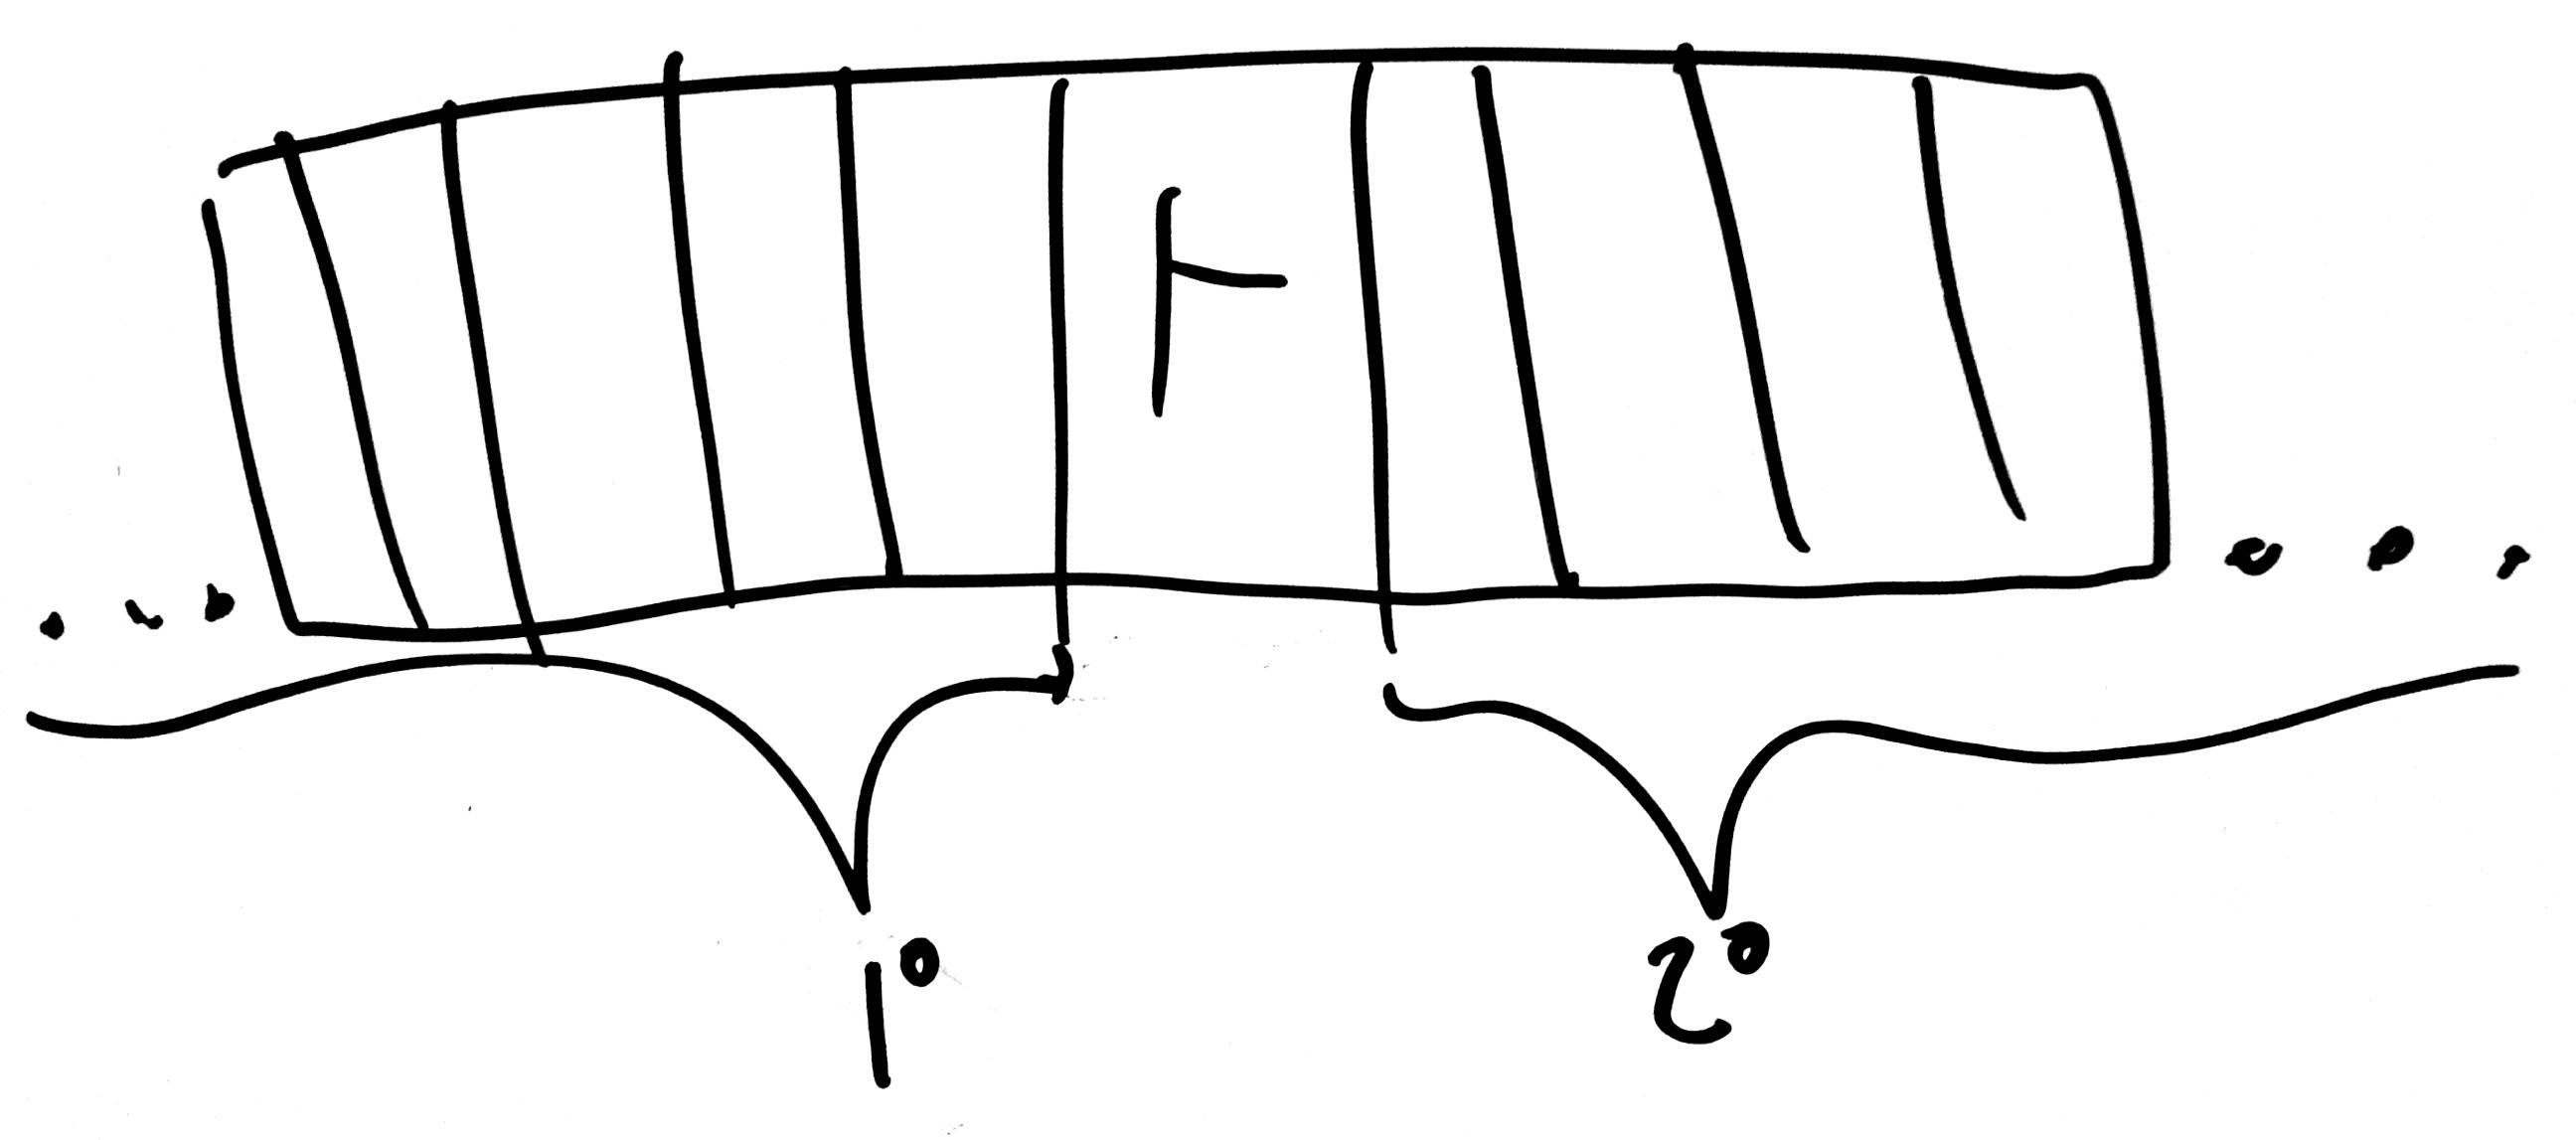
\includegraphics[width=220pt]{./images/img1.JPG}\\
           		\end{itemize}
           		Se deja en desuso la primer mitad de la cinta de B y la segunda mitad se utiliza para imitar a toda la cinta de A, el cabezal de B imita exactamente los movimientos de A.

           		
           \textbf{Imitando a B con A:}\\
           		Sean las siguientes máquinas de Turing:\\
           		\begin{itemize}
           			\item Máquina A como:\\
           				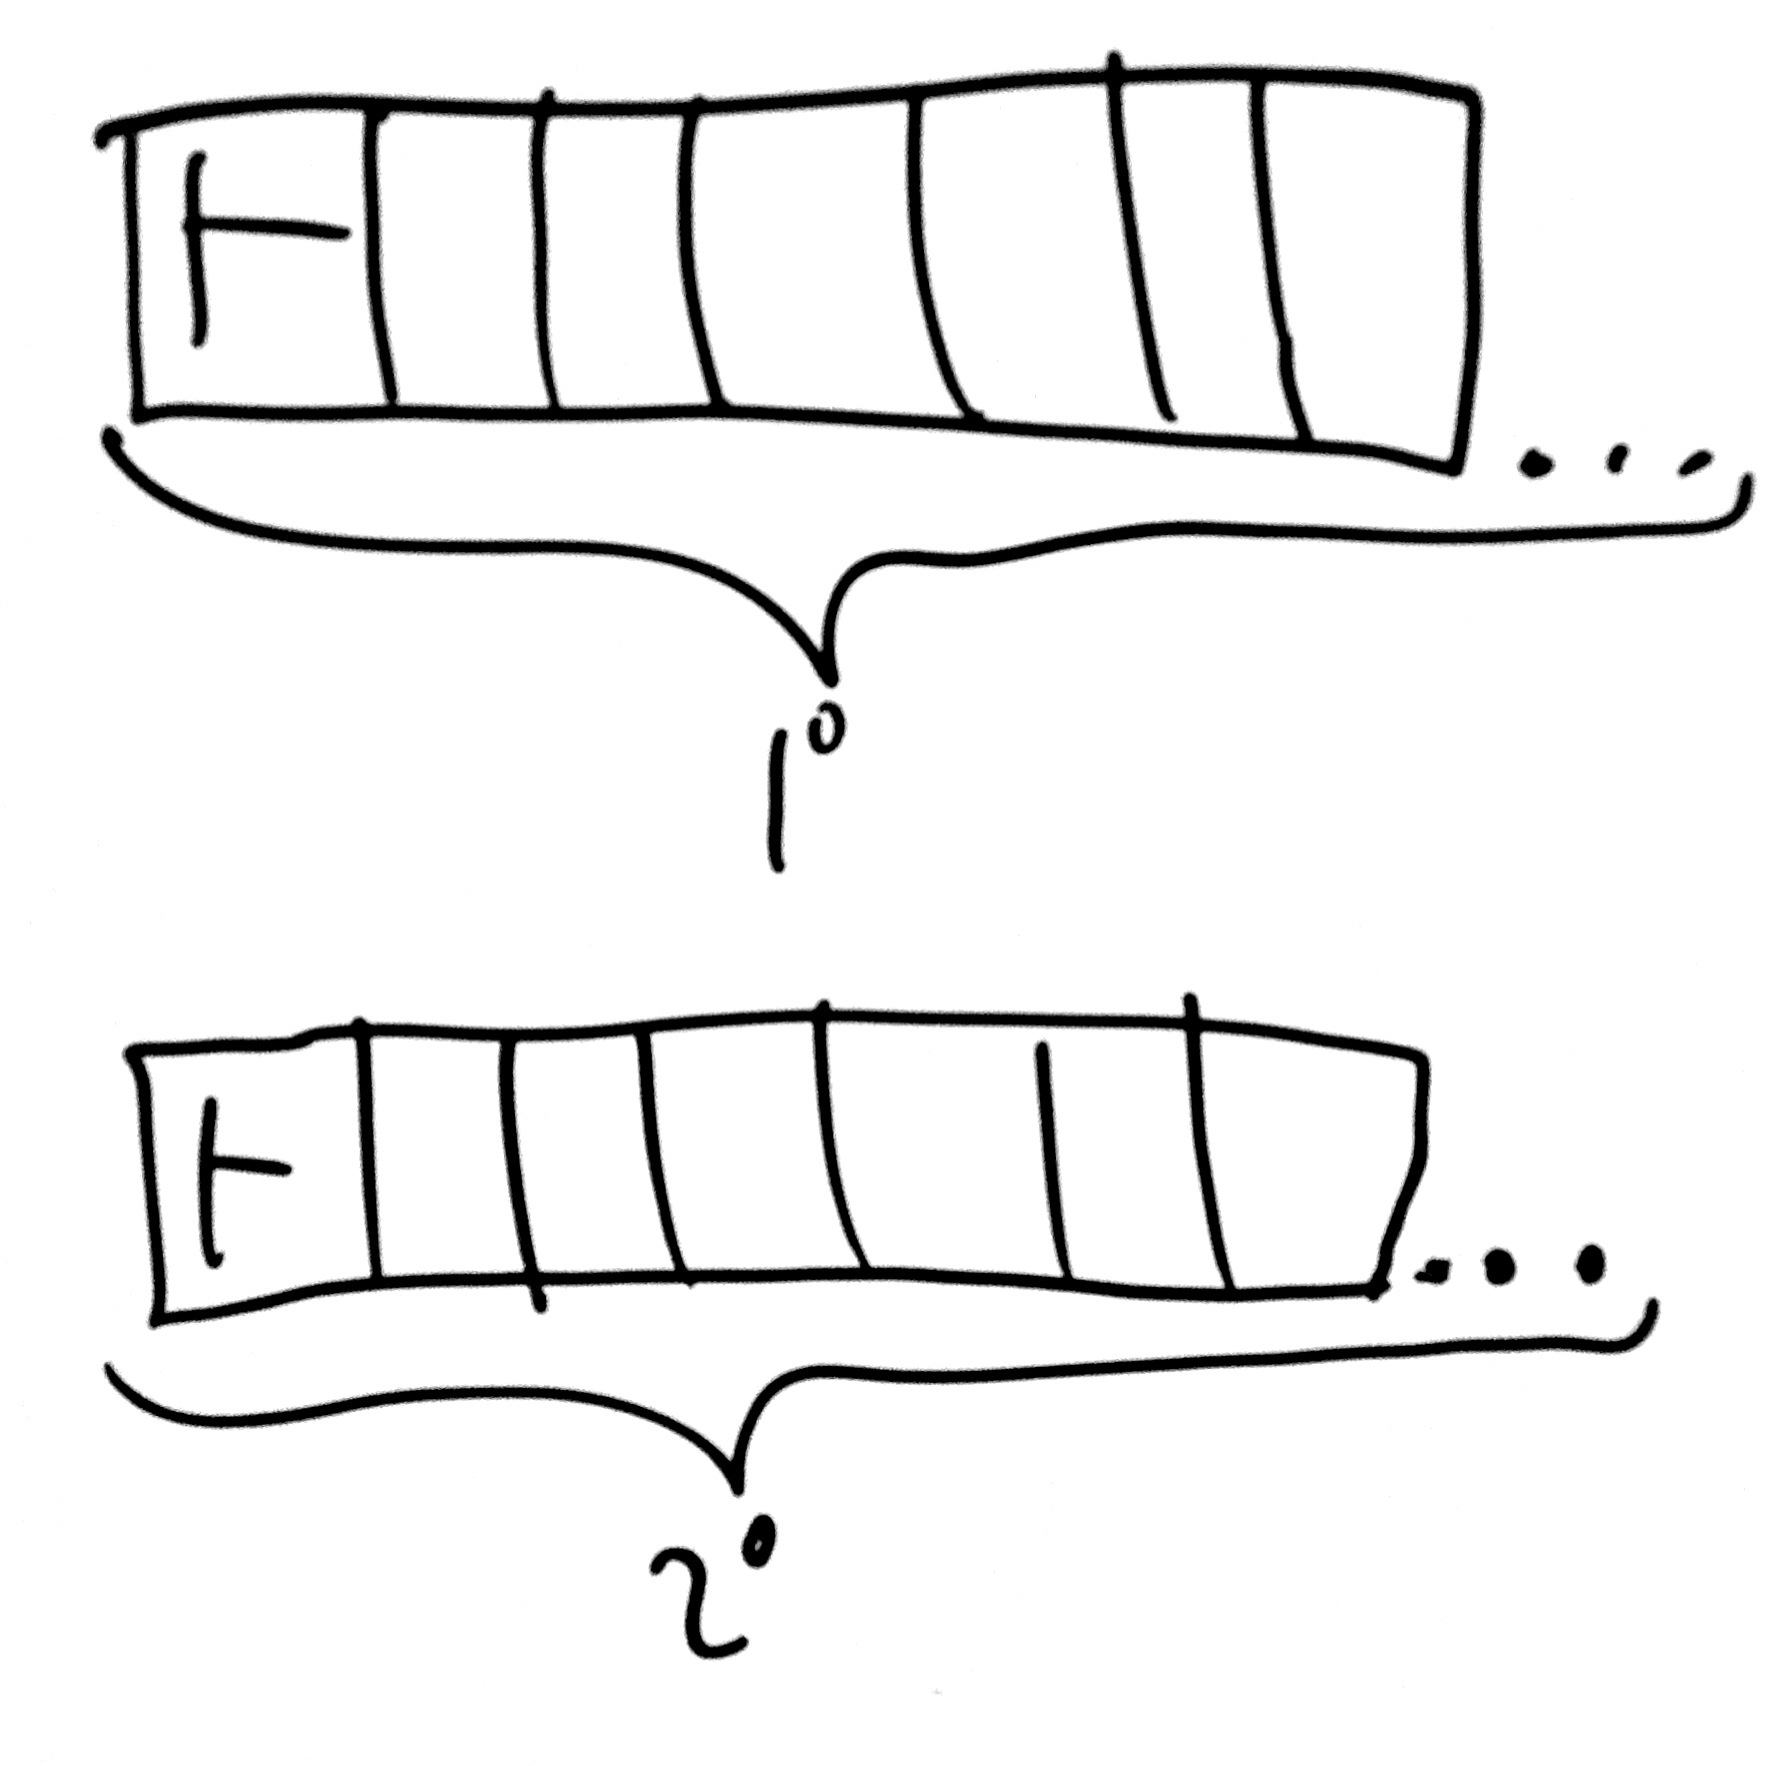
\includegraphics[width=120pt]{./images/img2.JPG}\\
           			
           			\item Máquina B vista como:\\
           				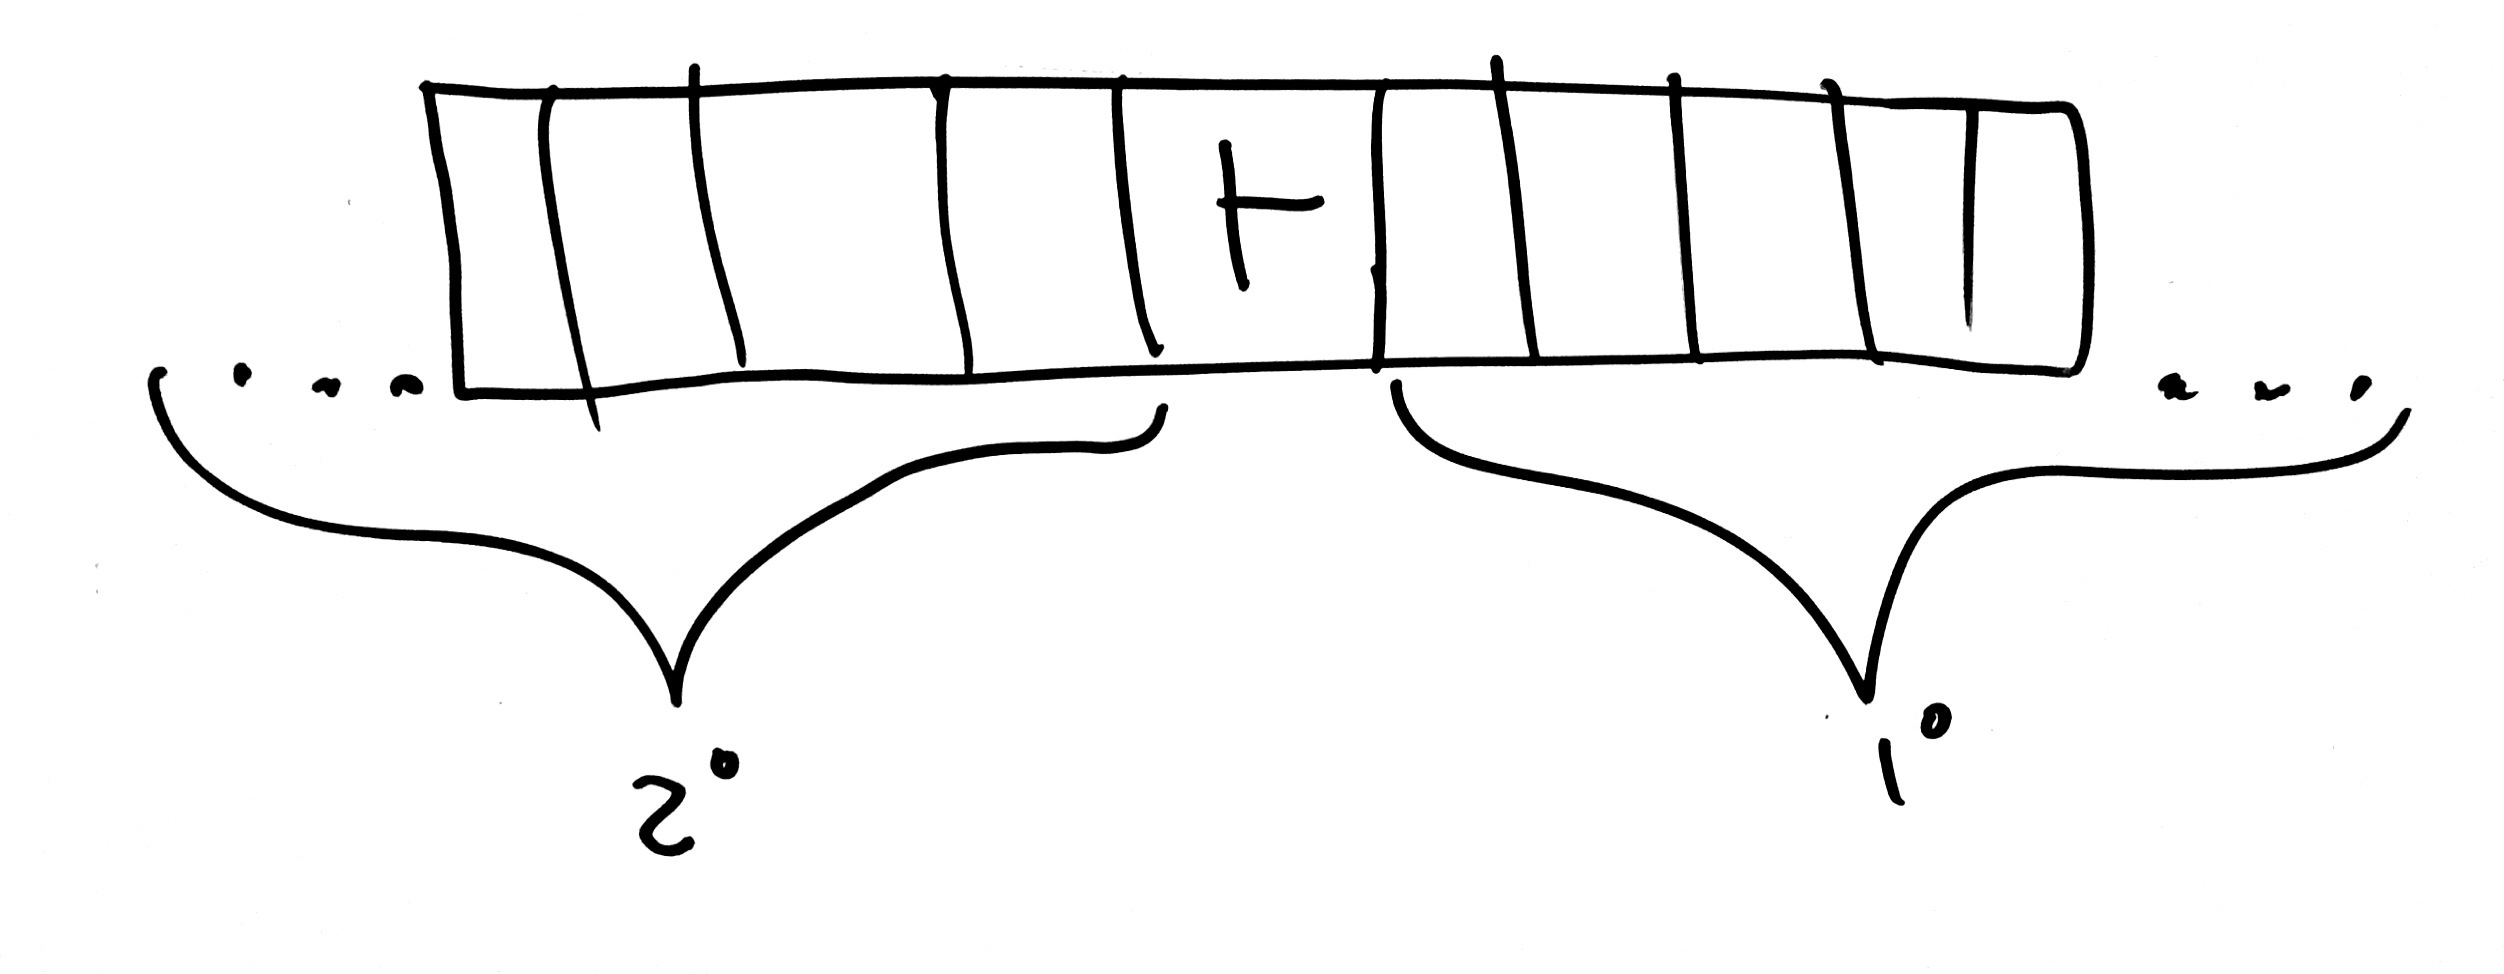
\includegraphics[width=220pt]{./images/img3.JPG}\\
           		\end{itemize}
           		En la primera mitad de B se puede operar con el cabezal desde $\vdash $ hacia la derecha sin restricciones, siendo esta primera mitad simulada por la primera cinta de A. Si de derecha a izquierda se llega a $\vdash$ en B será como llegar al símbolo inicial $\vdash$ de la primera cinta de A, también la segunda mitad de B será simulada por la segunda mitad de A, por lo que el cabezal de A imitará de manera contraria los movimientos del cabezal de B.\\
           		
           		En resumidas cuentas, el cabezal de la primera mitad de A imita exactamente los movimientos del cabezal de B cuando este está en la primera mitad y cuando el cabezal de B está en la segunda mitad el cabezal de la segunda mitad de A imita de manera contraria los movimientos del cabezal de B.
           
           % Ejercicio 2.2
           \item Máquina con una cinta semi-infinita en la que cada celda puede
           reescribirse a lo más dos veces.\\
           \textit{Solución:}\\ 
           Sean A una máquina de Turing con una cinta semi-infinita y B una máquina de Turing semi-infinita en ambas direcciones. 
           		
           \textbf{Imitando a A con B:}\\
           		Sean las siguientes máquinas de Turing:\\
           		\begin{itemize}
           				\item Máquina A vista como:\\
           					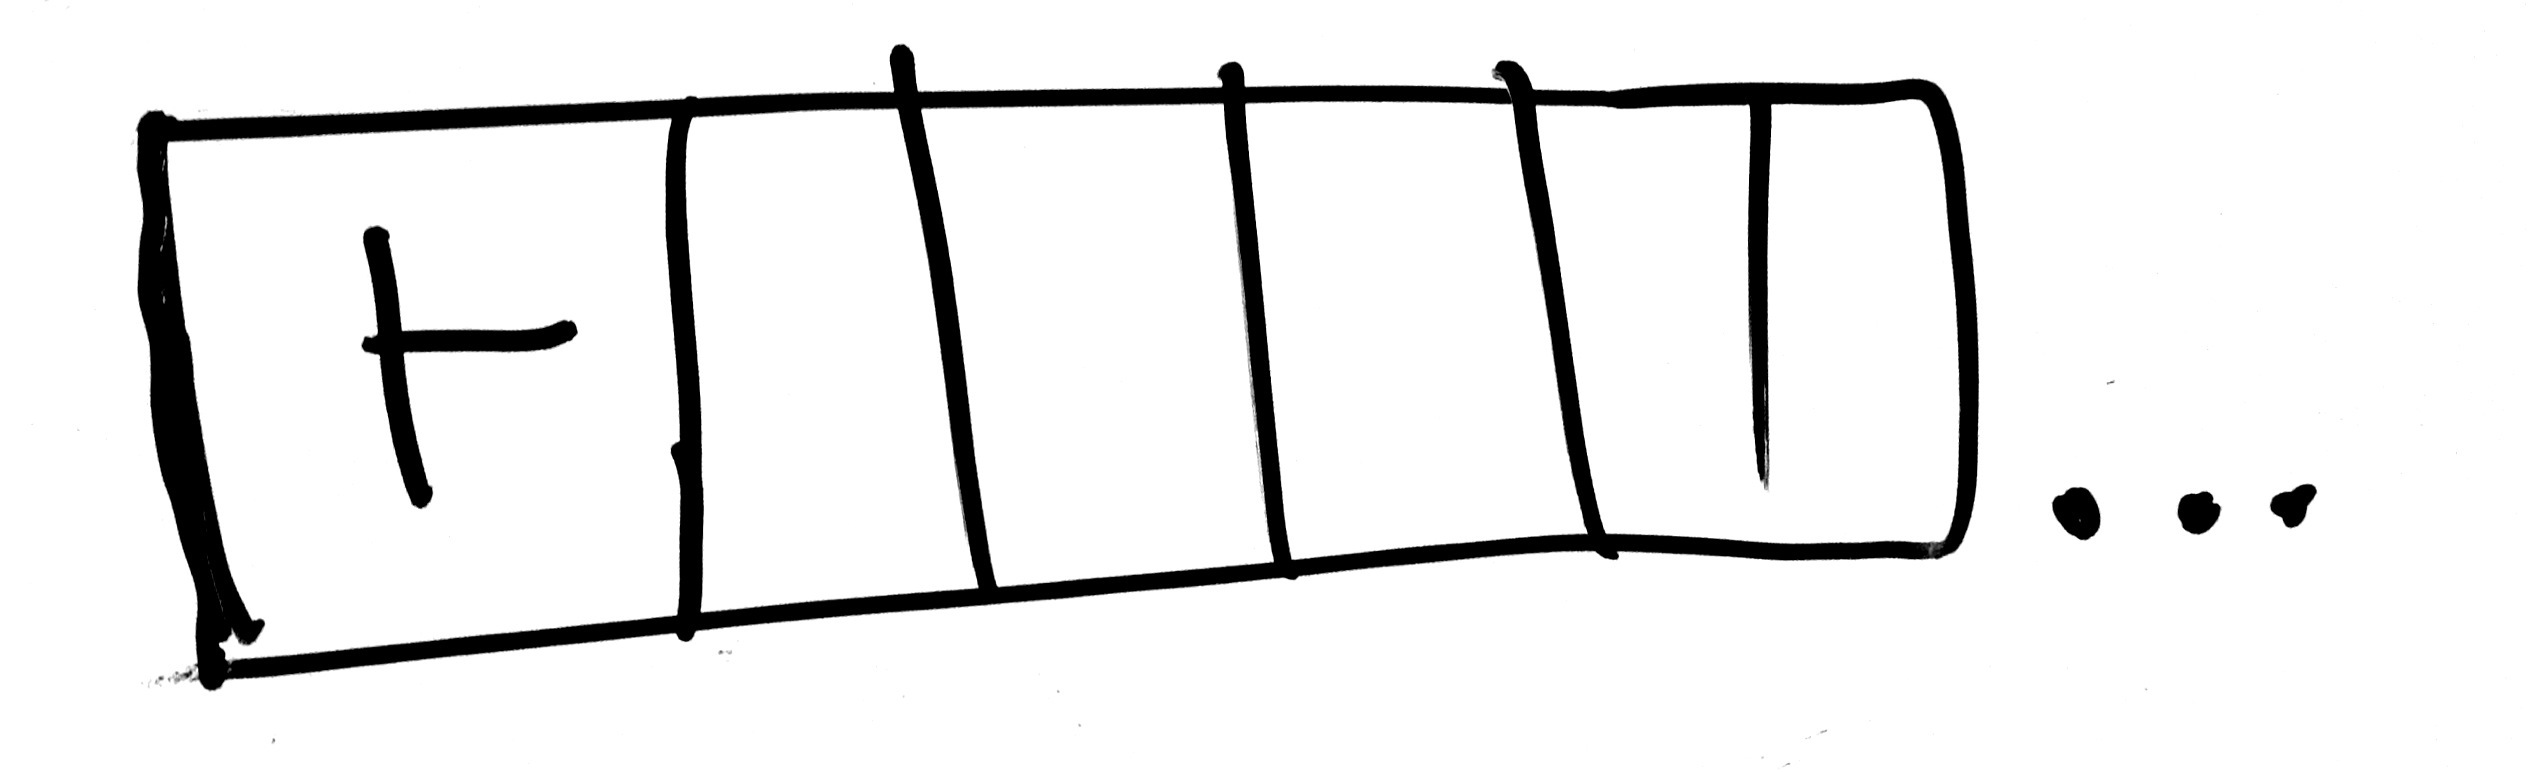
\includegraphics[width=150pt]{./images/img4.JPG}\\
           	
           				\item Máquina B vista como:\\
           					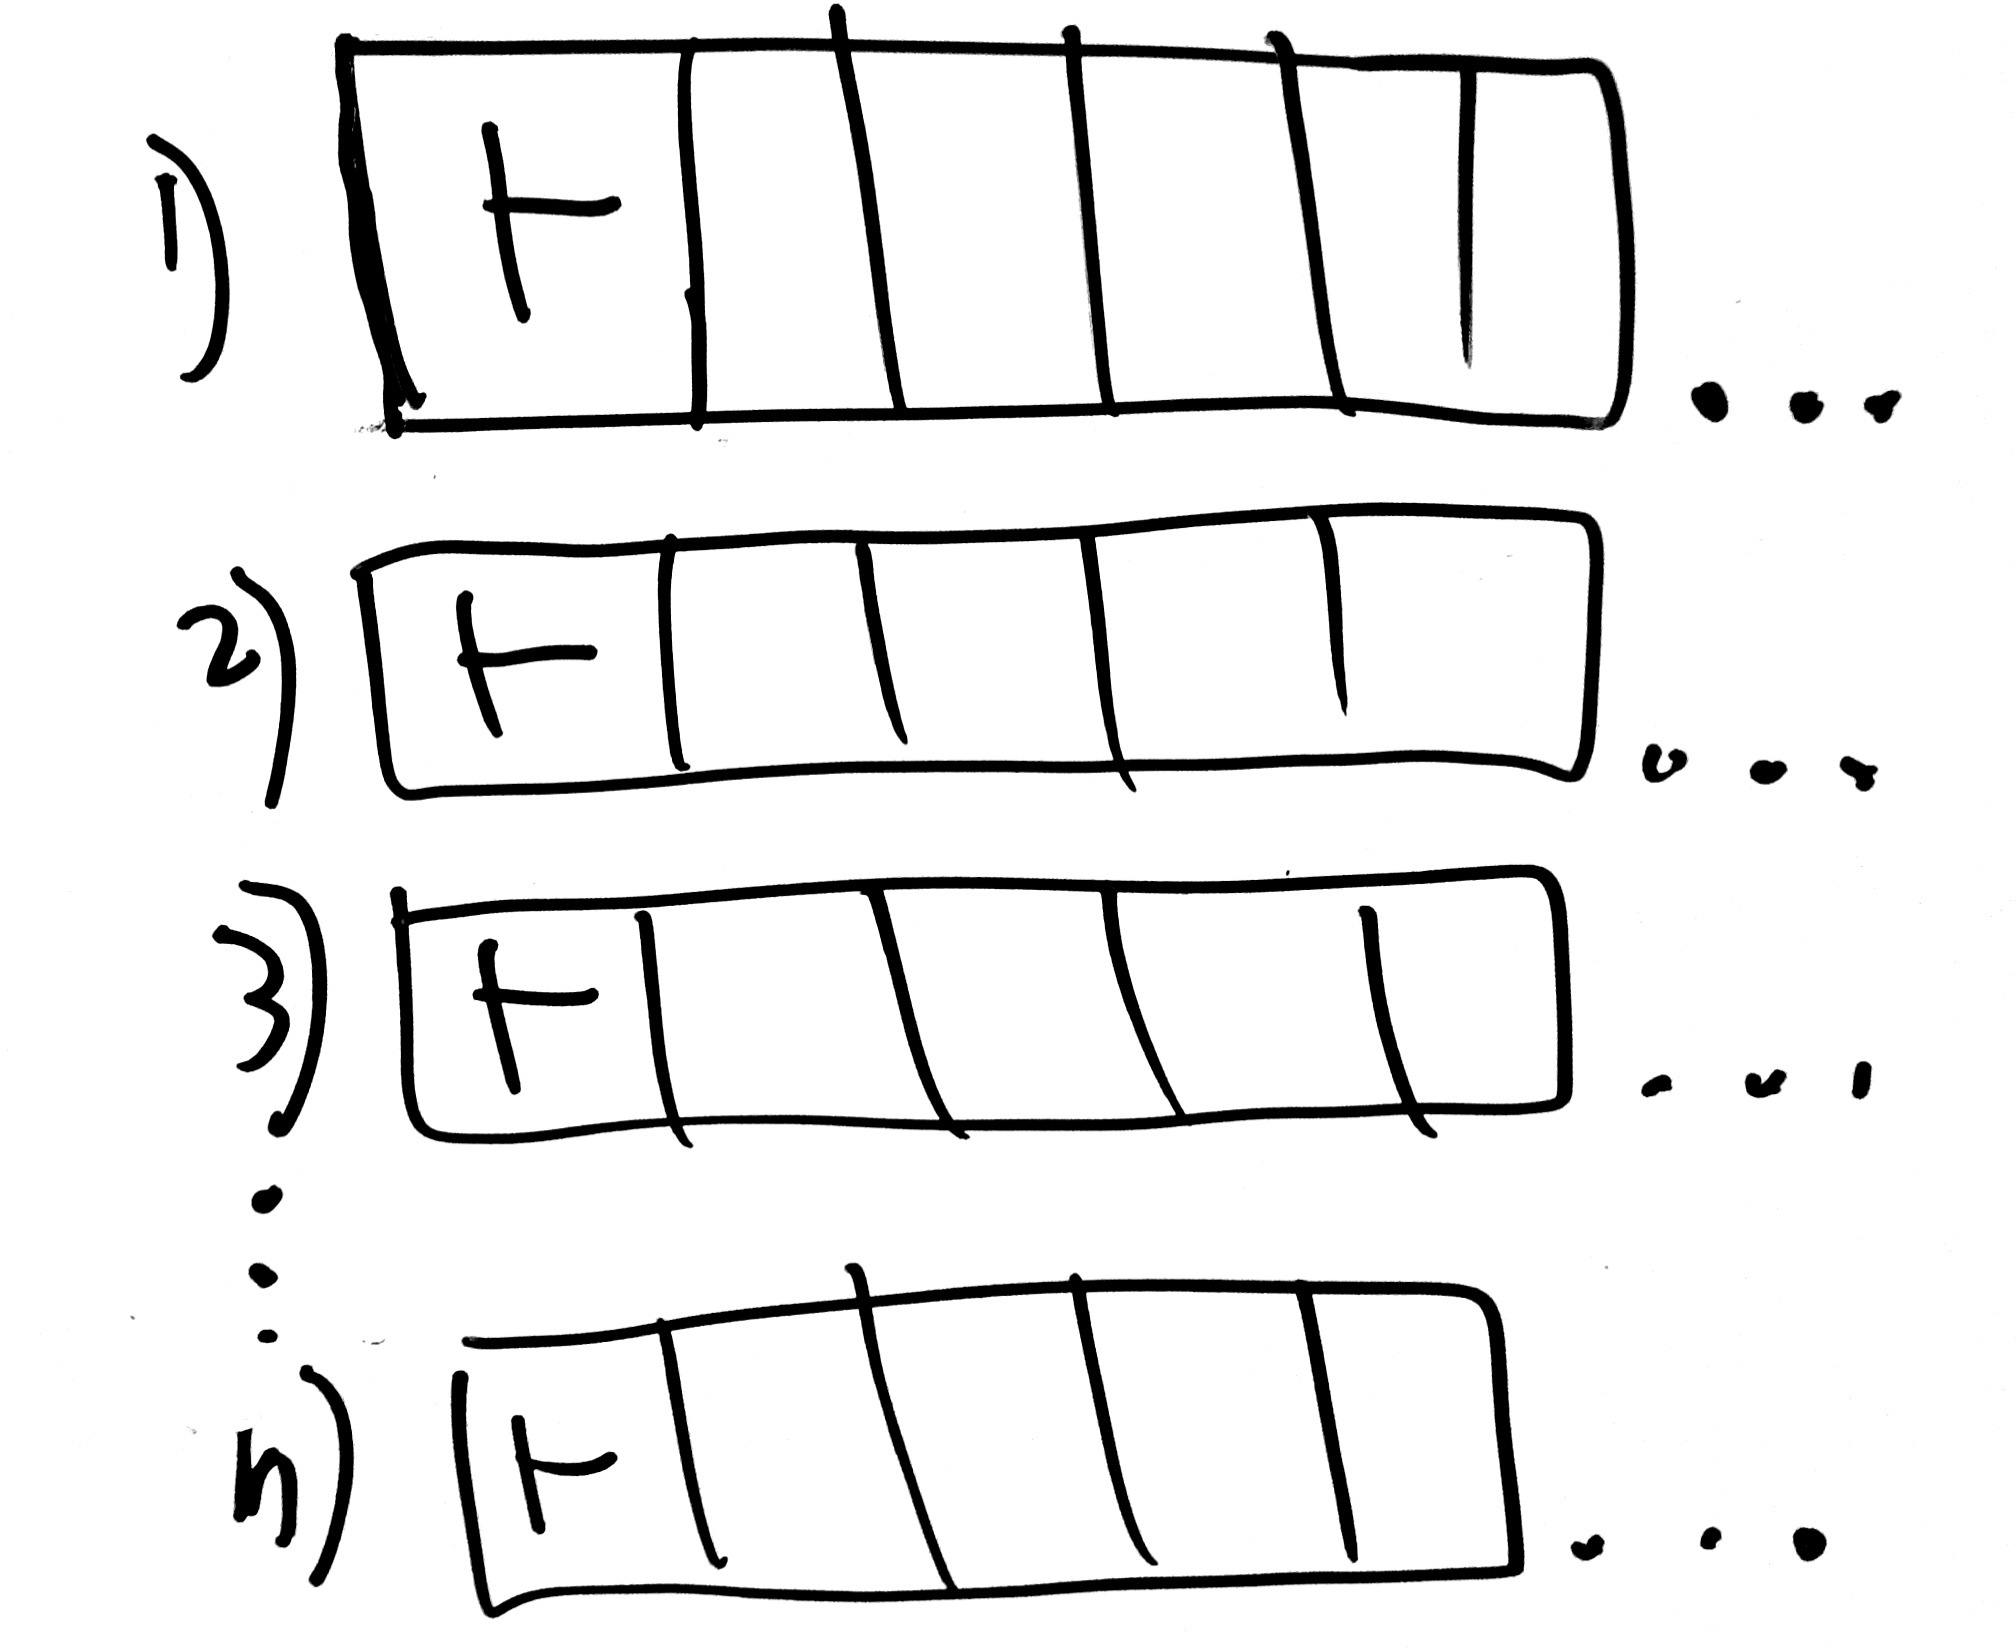
\includegraphics[width=150pt]{./images/img5.JPG}\\
           		\end{itemize}
           		Como B tiene n cintas, cada vez que se terminen las oportunidades de reescritura en alguna celda de cualquier cinta de B, podemos copiar todos los símbolos de la cinta en que se quiere reescribir y pegarlos en otra cinta en blanco, de esta forma se tendrán otras dos oportunidades de reescritura para esa celda. Se repite el mismo proceso de copiado para cada dos operaciones de reescritura en A y se sigue trabajando sobre la cinta con la copia más actual.
           		 
           \textbf{Imitando a B con A:}\\
           		Sean las siguientes máquinas de Turing:\\
           		\begin{itemize}
           			\item Máquina A vista como:\\
           				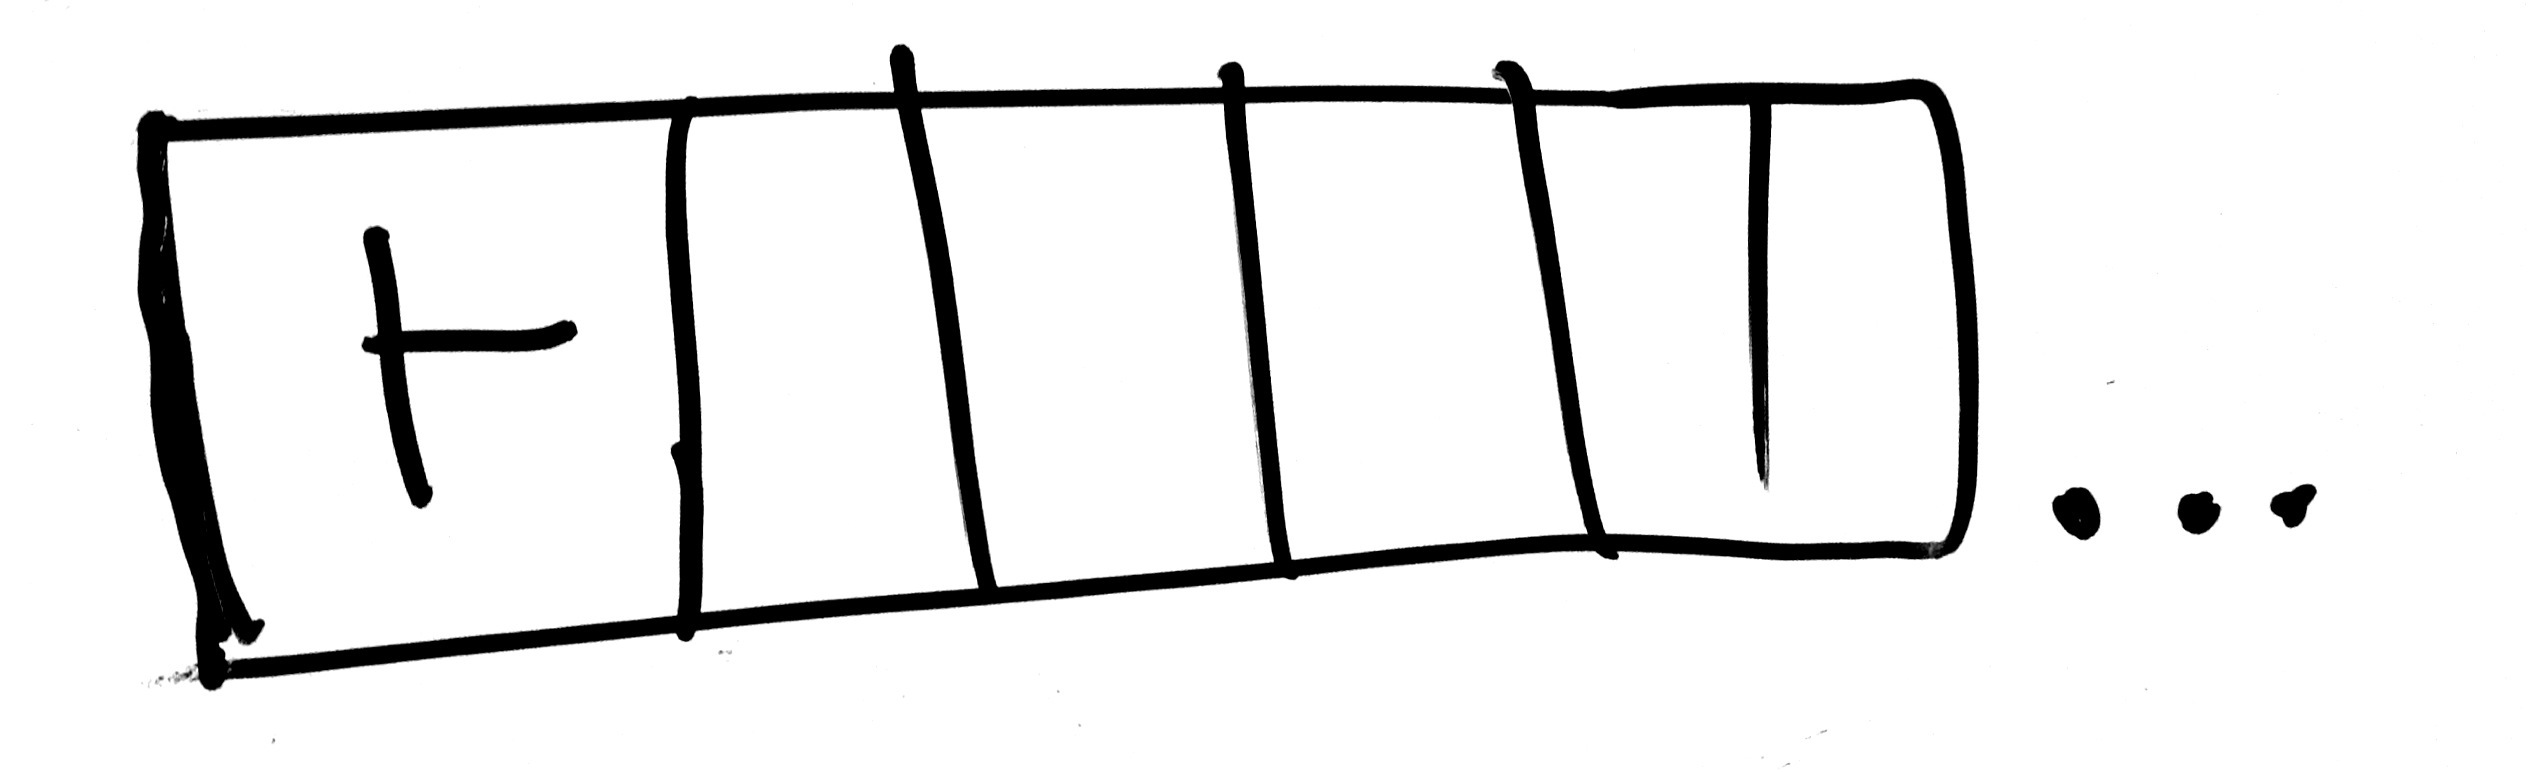
\includegraphics[width=150pt]{./images/img4.JPG}\\
           
          		\end{itemize}
          		En el alfabeto de la cinta de A se incluirá al símbolo * que servirá para saber cuántas reescrituras se han hecho en una casilla, cada vez que el cabezal quiera escribir en una casilla, el cabezal verifica si hay un * en la siguiente casilla a la que quiere escribir ó sobreescribir, y se comportará de la siguiente manera:
          		\begin{enumerate}
          			\item Si no hay un * en la siguiente casilla, entonces el cabezal procede a escribir, además recorre una casilla todos los elementos que están después de la casilla en la que escribió, en el hueco que queda escribe un * y regresa a la casilla donde escribió inicialmente a esperar la siguiente instrucción de escritura.
          			
          			\item En caso contrario se realiza alguno de los siguientes pasos
          			\begin{enumerate}
          				\item Si hay un * y en la siguiente casilla hay otro *, entonces se rechaza la escritura de la casilla sobre la que se quería escribir y el cabezal regresa a la casilla original donde quería escribir a esperar la siguiente instrucción.
          				
          				\item Si hay un * y en la siguiente casilla no hay otro *, entonces el cabezal procede a escribir además recorre una casilla todos los elementos que están después de la casilla en la que escribió, en el hueco que queda escribe un * y regresa a la casilla donde escribió inicialmente a esperar la siguiente instrucción de escritura.
          				
          			\end{enumerate}
          		\end{enumerate}
           
       \end{itemize}
       
       % Ejercicio 3.
       \item Da una definición formal de una máquina enumeradora y una 
       definición del lenguaje que enumera; y utilizando tu definición, describe
       una máquina enumeradora que imprima todos los números naturales.\\
       \textit{Solución:} Las definiciones propuestas son: 
       $\newtheorem{defi}{\it Definición}$
       \begin{defi}
           Una Máquina Enumeradora tiene un control finito y dos cintas: una
           cinta de trabajo para leer y escribir, y y una cinta de salida de
           sólo escritura. La cabeza de la cinta de trabajo puede moverse en
           cualquier dirección y puede leer y escribir cualquier elemento del
           alfabeto de la cinta. La cabeza de la cinta de salida se mueve 
           una celda a la derecha cuando escribe un símbolo, y sólo puede 
           escribir cadenas en $\Sigma$, separadas por el símbolo $\#$ . No 
           hay ningún estado de entrada ni de aceptación ó rechazo. La Máquina 
           Enumeradora comienza en su estado inicial con ambas cintas en blanco. 
           Se mueve según su función de transición, como una Máquina de Turing,  
           ocasionalmente escribiendo símbolos en la cinta de salida según lo 
           determinado por la función de transición. En algún momento puede 
           entrar en un estado de enumeración especial, que es sólo un estado 
           distinguido de su control finito. Cuando esto sucede, se dice que la 
           cadena actualmente escrita en la cinta de salida se enumera. La cinta 
           de salida se borra automáticamente y la cabeza de la cinta de salida
           se mueve de nuevo al principio de la cinta (la cinta de trabajo se
           deja intacta), y la máquina continúa desde ese punto. La Máquina
           Enumeradora funciona para siempre.
       \end{defi}
       
       \begin{defi}
           El lenguaje que enumera $L(E)$ se define como el conjunto de todas
           las cadenas en $\Sigma^{*}$ que se enumeran siempre por la 
           Máquina de Enumeración $E$, entre un par de $\#s$. La máquina podría 
           nunca entrar en su estado de enumeración, en cuyo caso $L(E) = \varnothing$,
           o podría enumerar infinitamente muchas cadenas. La misma cadena
           se puede enumerar más de una vez. 
       \end{defi}
       
       Ahora bien, describamos una Máquina Enumeradora E que imprima todos los
       números naturales. \\
       Se fija un órden canónico para $\Sigma^{*}$ de la siguiente manera: se listan 
       las cadenas por órden de tamaños, cadenas del mismo tamaño en "órden numérico".
       Es decir, sea $\Sigma = \{a_0, a_1, ..., a_{k-1}\}$ y $a_i$ es el "dígito" $i$
       en base $k$. Entonces las cadenas de longitud $n$ son los números de $0$ a
       $k^{n}-1$ escritos en base $k$. \\ 
       Entonces, siendo $\Sigma = \{0, 1\}$, el órden canónico es $\epsilon$, $0$, $1$,
       $00$, $01$, $10$, $11$, $000$, $001$, $...$ (así es como se debería de ver la
       cinta de salida). \\
       Notemos que el orden es aparentemente simple en el cual se generan las
       representaciones más cortas de $0$, $1$, $2$, $...$ en base $k$ $...$ Por lo
       que nos generará todos los números naturales.
       
       % Ejercicio 4.
       \item Muestra que es posible simular un $AFD$ utilizando una máquina
       de Turing determinista (puedes usar alguna variante de la máquina de
       Turing siempre y cuando sea determinista).\\
            \textit{Solución:}\\
       			Para simular un $AFD$ se utilizará una máquina de Turing con cuatro cintas denominadas A,B,C y D, las cuales no se alteran y sólo sirven de lectura. A continuacuón se describe cada cinta:
       			\begin{enumerate}[A)]
       				\item Esta cinta servirá para leer la cadena de entrada Del $AFD$. 
       				
       				\item Almacena los estados del $AFD$ y sólo simula la transición entre estados del $AFD$ por medio del cabezal. Para mayor comodidad los estados $q_i$ se verán como símbolos del alfabeto de la cinta. 
       				
       				\item Cada casilla de esta cinta concide con la posición de las casillas que están en la cinta B, por lo que esta cinta sirve para indicar los estados a los que va el estado $q_i$ en la casilla $i$ de B en caso de que se lea algún símbolo $1$ en A, de esta menera la cinta D sirve para indicarle al cabezal de B hacia donde moverse cuando el cabezal de A ve el símbolo $1$ 
       				
       				\item Esta cinta tiene el mismo uso que la cinta C, pero ésta es para el caso del símbolo $0$.
       			\end{enumerate}
       			
       			Básicamente se copia en cada casilla de A los símbolos de la cadena que recibe el $AFD$, después en B se copian todos los estados del $AFD$, luego en C se pone en cada casilla el estado (casilla) al que se debe mover el cabezal de B en caso de que el cabezal de A lea un $1$, en D se hace lo mismo pero para cuando el cabezal de A lea un $0$.\\ 
       			
       			Hay que aclarar que los estados finales de la máquina de Turing están determinados por los mismos estados finales del $AFD$ y al referirnos que el cabezal de B se mueve al estado $q_i$ significa que el cabezal de B se pone a buscar en la cinta B el estado deseado $q_i$.\\
       			
       			\newpage
       			A continuación se muestra un ejemplo de como se vería la máquina de turing y sus cintas a partir de un $AFD$ dado:\\ \\ \\
       				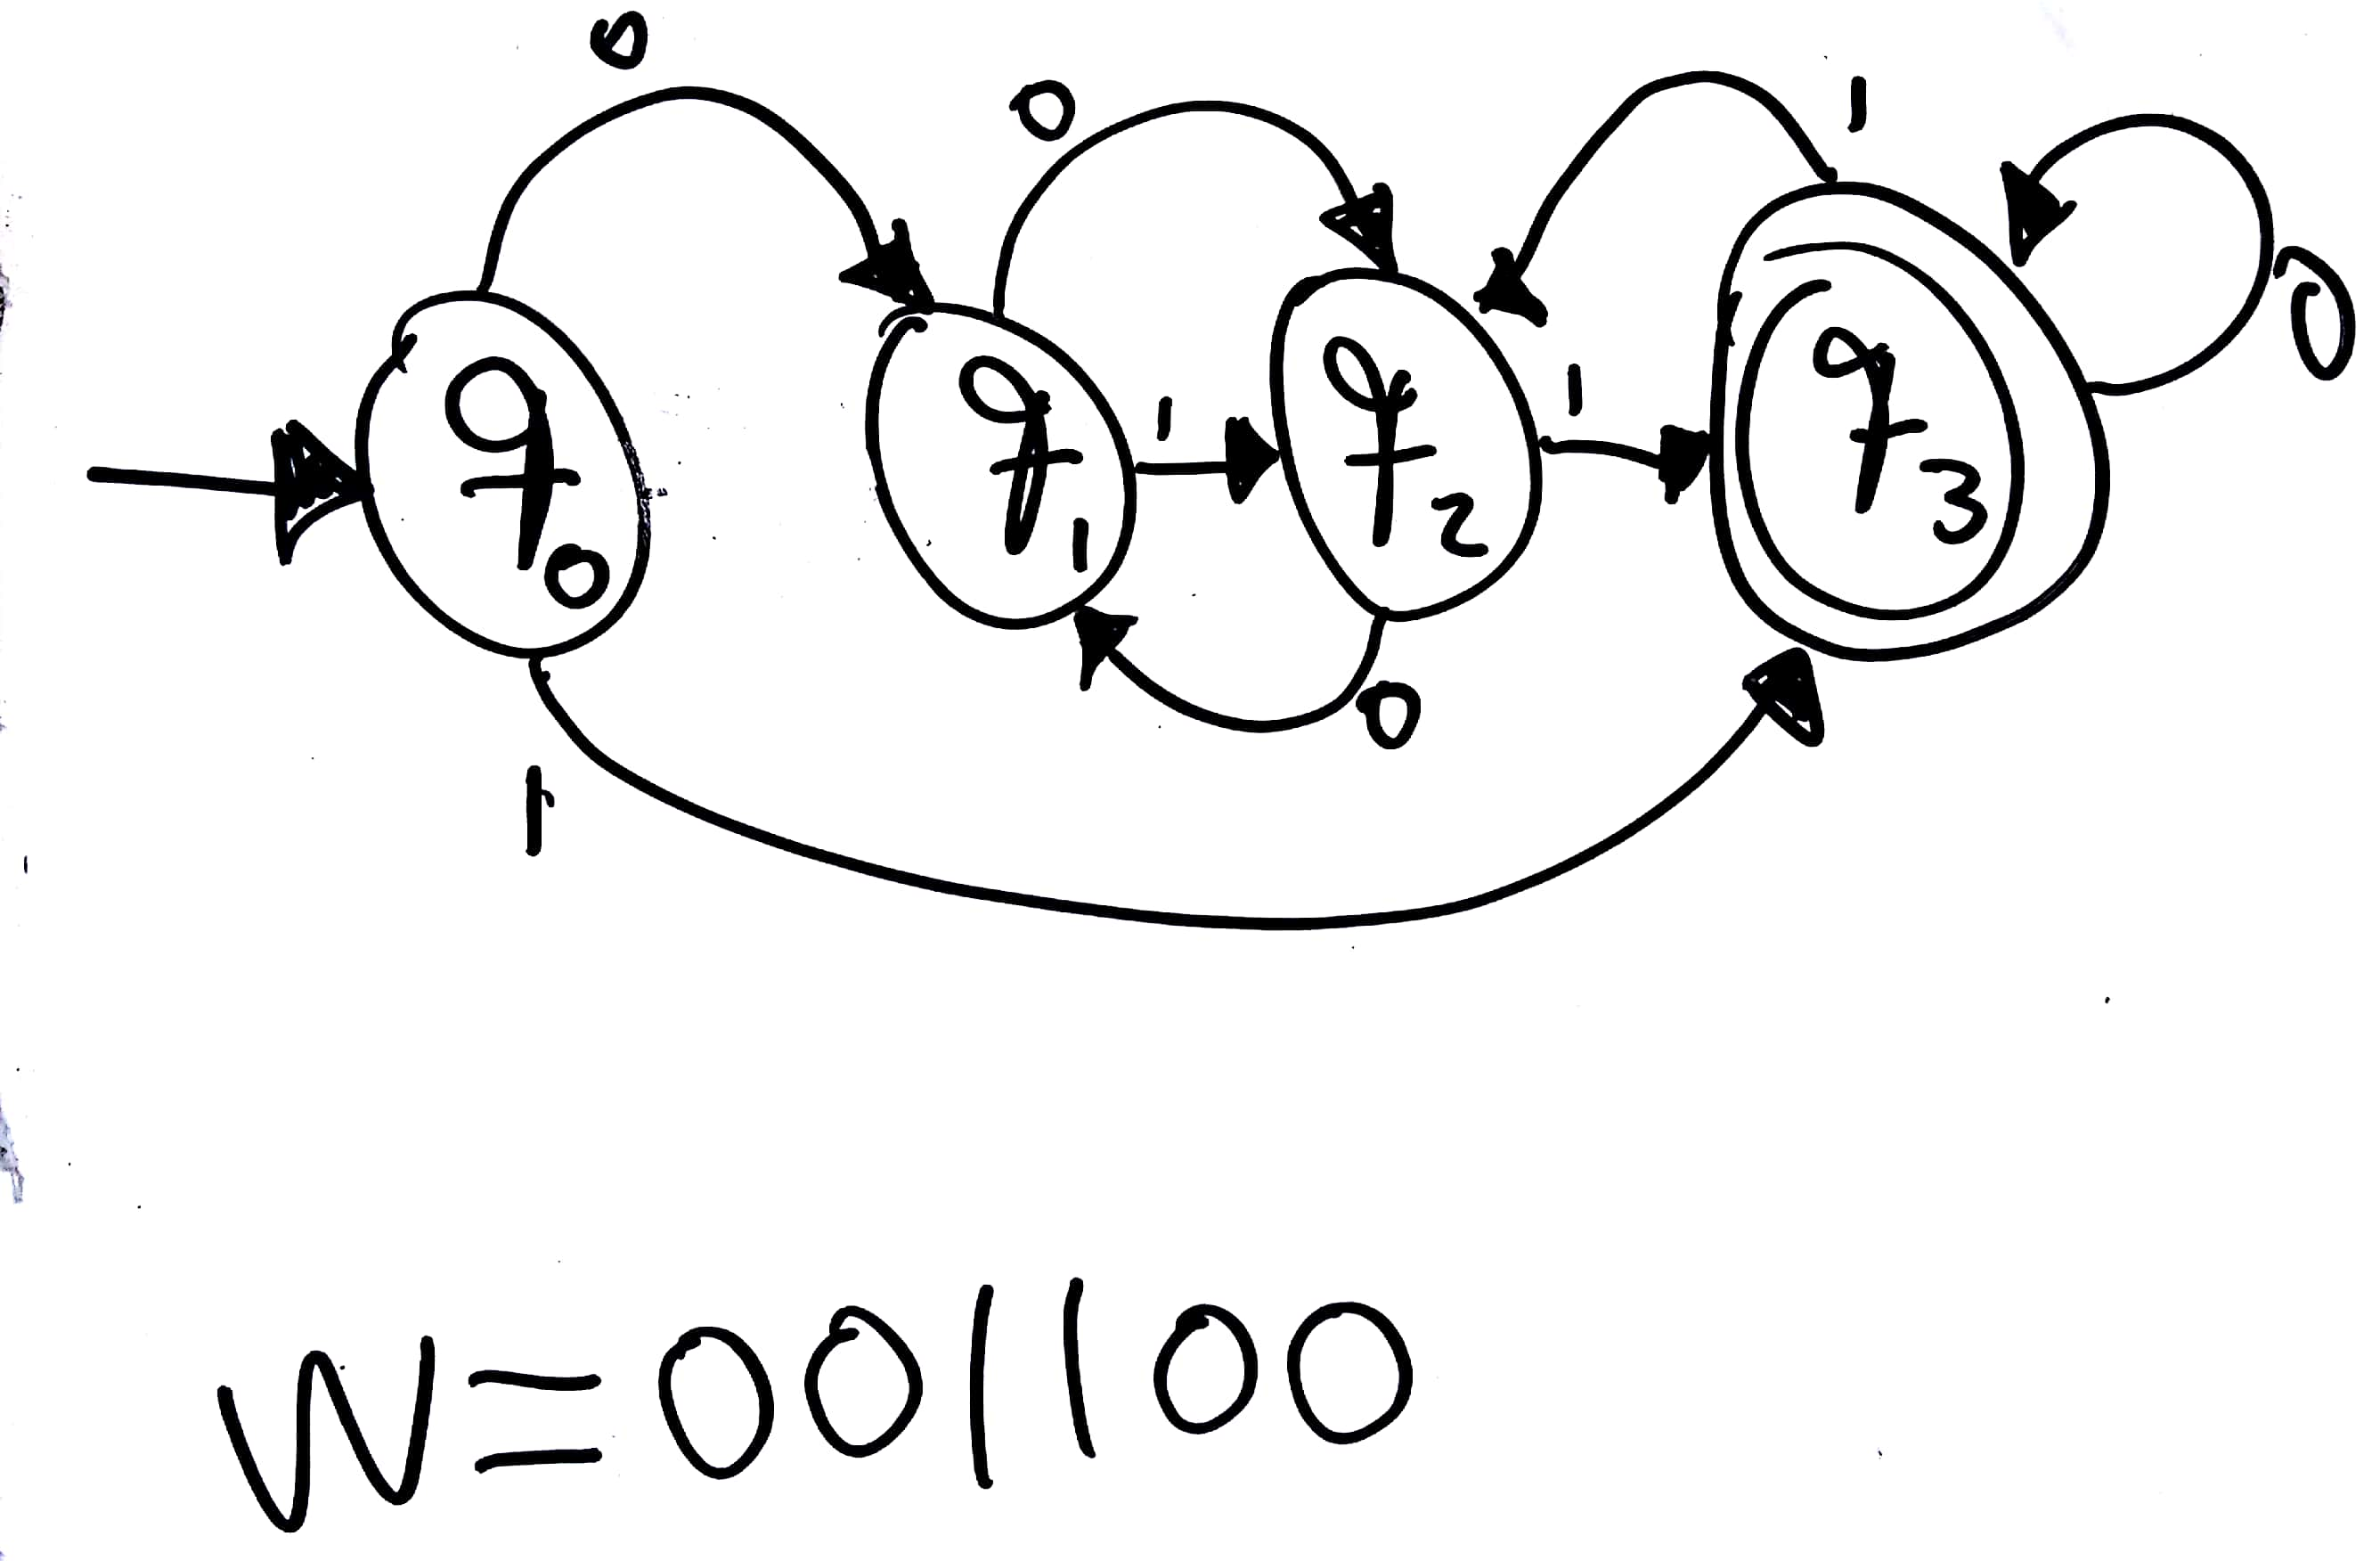
\includegraphics[width=250pt]{./images/img7.JPG}\\
       				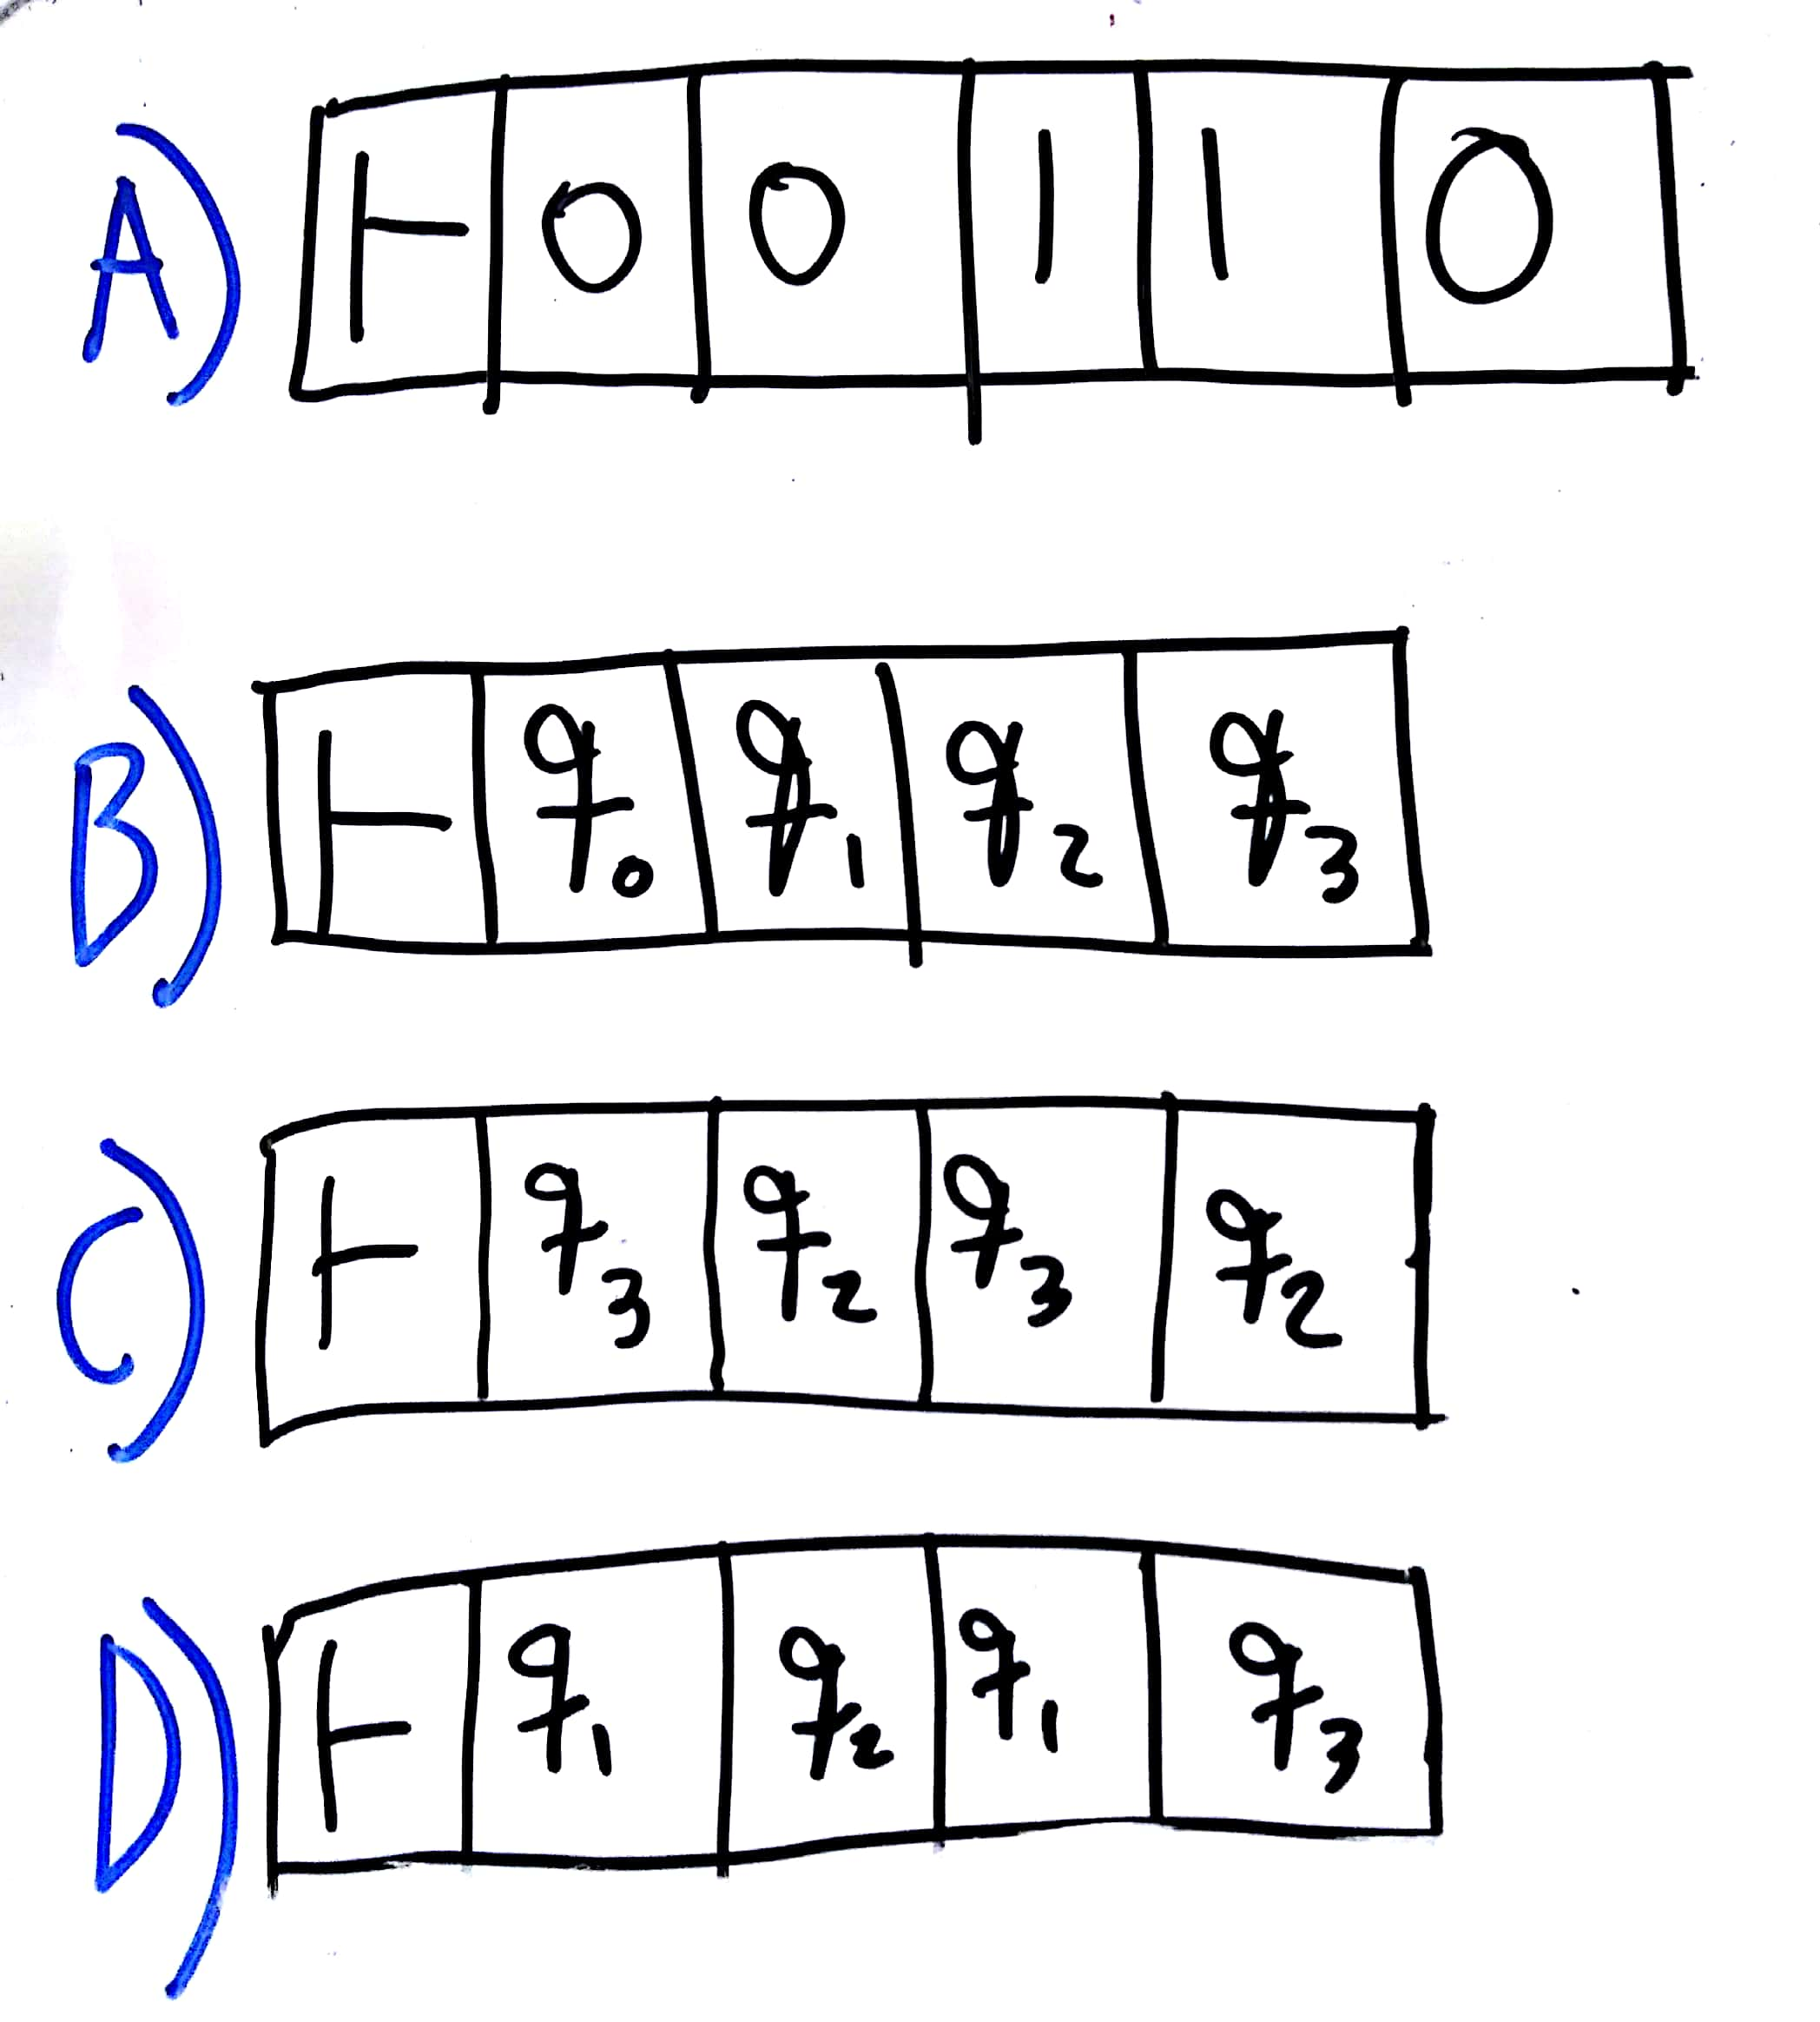
\includegraphics[width=150pt]{./images/img8.JPG}\\
       
       
       % Ejercicio 5.
       \item ¿Es posible simular un $APN$ con una máquina de Turing? De ser 
       posible, explica brevemente cómo sería la simulación. En caso contrario,
       argumenta tu respuesta. \\
       \textit{Solución:} Sí es  posible. Un Autómata de Pila se simula con una
       Máquina de Turing no determinista de dos cintas que utiliza dos cabezas
       lectoras (una para cada cinta): 
       \begin{itemize}
           \item Cinta 1. Corresponde a los símbolos de la cadena recibida como
           entrada. Es de solo lectura y se mueve únicamente a la derecha.
           \item Cinta 2. Corresponde a los símbolos en la pila. Para añadir
           un elemento a la pila, entonces escaneamos hacia la derecha,
           reemplazando los espacios en blanco por símbolos. Para eliminar
           un elemento en la pila, escaneamos hacia la izquierda y reemplazamos
           los símbolos por espacios en blanco.
       \end{itemize}
       
       Notemos que el tope de la pila se encontrará en la derecha de la segunda
       cinta, por lo que ésta nos sirve de almacenamiento. Además, los estados
       del Autómata de Pila se ``reutilizan'' en la Máquina de Turing, así como
       el alfabeto de la Pila.
       
       \newpage
       % Ejercicio 6.
       \item Da una codificación para las máquinas de Turing sobre un alfabeto
       binario. Además, muestra un ejemplo usando tu codificación.\\
            \textit{Solución:}\\
       			La codificación de una máquina de Turing queda de la siguiente manera:\\
       			\begin{itemize}
       				\item $Q=\{ q_1,q_2,...,q_r\}$, con $q_1$ el estado inicial, $q_2$ el único estado final y los estados que van de $q_3$ a $q_r$ son estados cualesquiera.\\
       				Los estados se codifican como $q_i = 0^i$.
       				
       				\item $\Gamma=\{x_1,x_2,x_3\}$, donde\\
       					$x_1 = \sqcup$ y se codifica como $0$\\
       					$x_2=0$ y se codifica como $00$\\
       					$x_3=1$ y se codifica como $000$\\
       					
       				\item Desplazamiento del cabezal: El desplazamiento del cabezal se codifica como
       					\begin{itemize}
       						\item $\leftarrow= 0$
       						\item $\rightarrow=00$
       						\item $\sqcup = 000$
       					\end{itemize} 
       				Con $\leftarrow , \rightarrow , \sqcup  \in D$
       				\item La codificación de la transición $\delta$ queda definida por
       					\begin{itemize}
       						\item $w_m=\delta(q_i,x_j)=\delta(q_k,x_h,d_n)$
       						\item Se pone un $1$ de separación entre cada elemento de la $\delta$
       						\item Al final de una transición se pone $11$ para indicar el fin de la transición.
       						\item De manera esquemática la codificación de la $\delta$ queda definida de la siguiente manera:\\
       							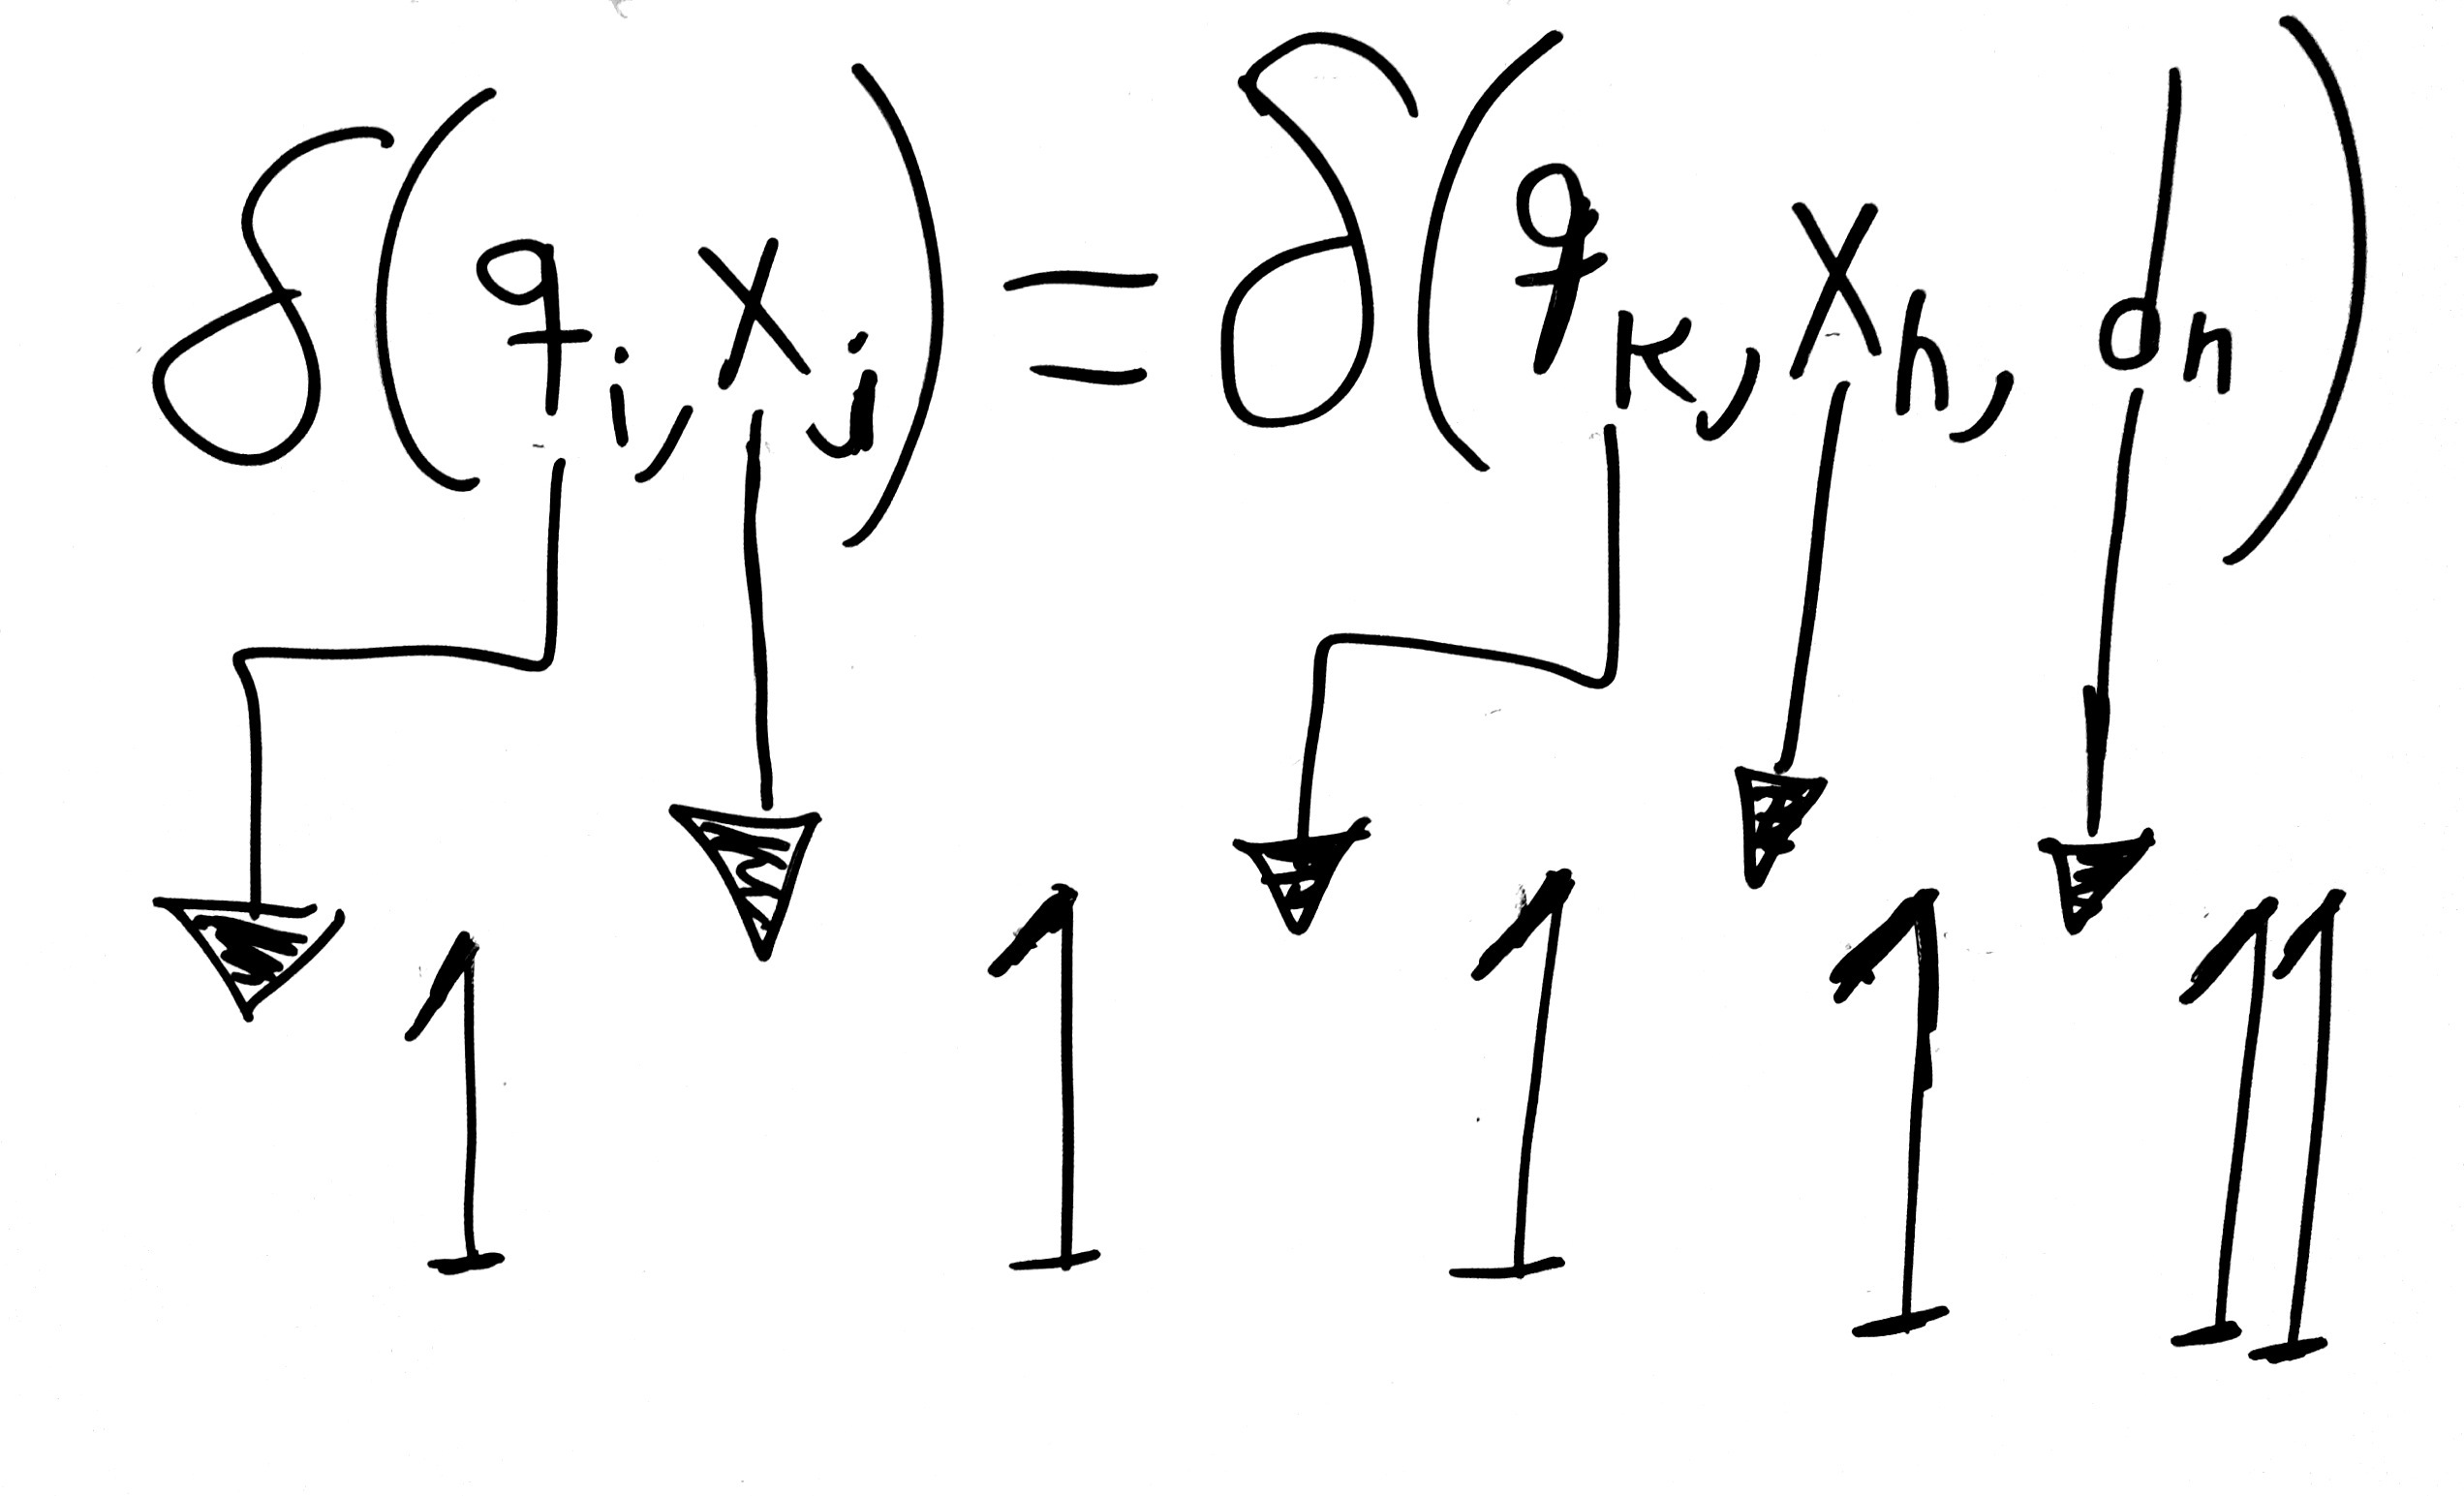
\includegraphics[width=220pt]{./images/img6.JPG}\\
       						 
       					\end{itemize}
       				\item La codificación completa de la máquina de Turing queda determinada por la concatenación de sus transiciones\\
       					$w_1w_2w_3...w_n$
       					
       			\end{itemize}
       			\textbf{Ejemplo:}\\
       				Sea M una  máquina de Turing definida por:
       				\begin{itemize}
       					\item $\delta (q_1,a) = \delta (q_2,a,\rightarrow)$
       					\item $\delta (q_2,b) = \delta (q_3,a,\rightarrow)$
       					\item $\delta (q_3,b) = \delta (q_1,b,\sqcup)$
       				\end{itemize}  
       				Con
       				\begin{itemize}
       					\item $\Sigma = \{a,b\}$
       					\item $Q=\{q_1,q_2,q_3\}$
       				\end{itemize}
       				
       				\newpage
       				La codificación de M queda de la siguiente manera:\\
       				\begin{itemize}
       					\item $q_1=0$
       					\item $q_2=00$
       					\item $q_3=000$
       					\item $\sqcup = 0$
       					\item $a=00$
       					\item $b=000$ 
       					\item $\delta (q_1,a) = \delta (q_2,a,\rightarrow) = 010010010010011$
       					\item $\delta (q_2,b) = \delta (q_3,a,\rightarrow) =001000100010010011$
       					\item $\delta (q_3,b) = \delta (q_1,b,\sqcup) =0001000101000100011$
       				\end{itemize}
       			La codificación final queda así:
       				$$010010010010011 001000100010010011 0001000101000100011$$
       
       % Ejercicio 7.
       \item Demuestra que el lenguaje $\{\langle M \rangle$ $|$ $M$ es
       una $MT$ total\} no es recursivamente enumerable y tampoco lo es 
       su complemento.
       \begin{proof}
           % Primera demosgtración.
           Sean $HALT_{TM} = \{\langle M, w \rangle$ $|$ $M$ es
           una $MT$ y $M$ se detiene con la entrada $w$\} y el lenguaje
           $TOTAL_{TM} = \{\langle M \rangle$ $|$ $M$ es una $MT$ total\}. 
           Veamos que $\overline{HALT_{TM}} \leq_m TOTAL_{TM}$. Sea 
           $f(\langle M, w \rangle) = \langle M_{T} \rangle$ una función
           computable definida de la siguiente forma: \\
           En la entrada $\langle M, w \rangle$
           \begin{itemize}
               \item Construye una Máquina de Turing $M_{T}$: 
               Para la entrada $x$:
               \begin{itemize}
                   \item [i)] Ejecutamos $M$ con la entrada $w$ hasta un máximo
                   de $|x|$ pasos.
                   \item [ii)] Si $M$ se ha detenido, entonces se cicla. Si $M$
                   aún no se ha detenido, entonces se
                   detiene (no se sabe si aceptando o
                   rechazando).
               \end{itemize}

           \end{itemize}
           
           La salida es $\langle M_{T} \rangle$.\\ \\
           Así, $\langle M, w \rangle \in \overline{HALT_{TM}}$
           $\Longleftrightarrow$ $f$ se detiene en todas las entradas
           $\Longleftrightarrow$ 
           $\langle M_{T} \rangle \in TOTAL_{TM}$. \\
           Finalmente, por un corolario visto en clase, como 
           $\overline{HALT_{TM}}$ no es recursivamente enumerable
           entonces $TOTAL_{TM}$ también lo es.\\
           
           % Segunda demostración.
           Ahora, veamos que $\overline{HALT_{TM}} \leq_m 
           \overline{TOTAL_{TM}}$. Sea $g(\langle M, w \rangle) =$
           $\langle M \rangle$ una función computable definida de la siguiente
           forma: \\
           En la entrada $\langle M, w \rangle$.
           \begin{itemize}
               \item Construye la Máquina de Turing $M$: Para la entrada $x$:
               \begin{itemize}
                   \item[i)] Ignoramos a $x$ y ejecutamos $M$ con $w$.
                   \item[ii)] Si $M$ acepta, entonces acepta. Si $M$ rechaza,
                   entonces rechaza. 
               \end{itemize}

           \end{itemize}
           
           La salida es $\langle M \rangle$. \\ \\
           Notemos que $g$ se detiene en todas las entradas o se cicla en todas
           las entradas. \\
           Así, $\langle M, w \rangle \in \overline{HALT_{TM}}$
           $\Longleftrightarrow$ $g$ se cicla en todas las entradas
           $\Longleftrightarrow$ 
           $\langle M \rangle \in \overline{TOTAL_{TM}}$. \\
           Por lo tanto, $\overline{HALT_{TM}} \leq_m \overline{TOTAL_{TM}}$.\\
           Finalmente, por un corolario visto en clase, como
           $\overline{HALT_{TM}}$ no es recursivamente enumerable entonces
           $\overline{TOTAL_{TM}}$ también lo es. \\
       \end{proof}
       
       \newpage
       % Ejercicio 8.
       \item Una máquina de Turing tiene un estado \textit{inútil} si la
       máquina nunca entra a dicho estado. Muestra que el lenguaje
       $\{\langle M \rangle$ $|$ $M$ es una $MT$ con un estado inútil\}
       es indecidible.
       \begin{proof}
       		La demostración se hará por reducción al absurdo.\\
       		Sea $INL=\{ \langle M \rangle$ $| M $ es una MT con un estado inútil $\}$\\
       		Suponer que $INL_{TM}$ es decidible, así que $\exists R$ una MT que decide a $INL_TM$.\\
       		Por otro lado podemos ver que para cualquier MT $M$ con por lo menos un estado de aceptación, que denominaremos $q$, se cumple que $q$ es un estado inútil $ \Leftrightarrow L(M)= \emptyset$\\
       		
       		A partir de lo anterior podemos usar a $R$ para decidir $E_{TM}$. Así que daremos una MT $S$ con entrada $\langle M \rangle$ y que la pasa $\langle M \rangle$ a $R$.\\
       		$S$ se comporta de la siquiente manera
       		\begin{itemize}
       			\item Corre $R$ con entrada $\langle M \rangle$.
       			\item Descide lo que decida $R$
       		\end{itemize}    
       		Si $S$ acepta , entonces $M$ tiene un estado inútil y $L(M)=\emptyset $ $!$, llegamos a una contradicción a causa de que estamos decidiendo a $E_{TM}$ determinando que $L(M)=\emptyset$ y sabemos que $E_{TM}$ es indecidible.\\
       		Por lo tanto $INL_{TM}$ es indecidible.
       		
       \end{proof}
       
       % Ejercicio 9.
       \item Muestra que el lenguaje $\{\langle M_1, M_2 \rangle$ $|$
       $M_1, M_2$ son $MT$ y $L(M_1) \neq L(M_2)\}$ es indecidible.
       \begin{proof}
           Sean $A_{TM} = \{\langle M, w \rangle$ $|$ $M$ es una
           $MT$ y $M$ acepta a $w$\} y $\overline{EQ_{TM}} = $ 
           $\{\langle M_1, M_2 \rangle$ $|$ $M_1, M_2$ son $MT$
           y $L(M_1) \neq L(M_2)\}$. Veamos que
           $A_{TM} \leq_m \overline{EQ_{TM}}$. Sea 
           $f(\langle M, w\rangle) = \langle M_1, M_2\rangle$  una función 
           computable definida de la siguiente forma: \\ \\
           En la entrada $\langle M, w \rangle$
           \begin{itemize}
               \item Construye la Máquina de Turing $M_1:$ rechaza todas las
              entradas.
               \item Construye la Máquina de Turing $M_2:$ Para la entrada $x$:
               \begin{itemize}
                   \item[i)] Ignoramos a $x$ y ejecutamos $M$ con $w$.
                   \item[ii)] Si $M$ acepta $w$, entonces acepta.
               \end{itemize}
            
           \end{itemize}
           
           La salida es $\langle M_1, M_2 \rangle$. \\ \\
           Observemos que $L(M_1) = \varnothing$. Para el lenguaje de 
           $M_2$: 
           \begin{itemize}
               \item Si $M$ acepta $w$ (i.e. 
               $\langle M, w \rangle \in A_{TM}$) entonces
               $L(M_2) \neq \varnothing$. Por lo tanto, 
               $L_(M_1) \neq L(M_2)$.
               \item Como $M$ no rechaza necesariamente a $w$, por definición 
               de $A_{TM}$, entonces $\langle M, w \rangle \notin A_{TM}$,
               por lo que $L(M_2) = \varnothing$. Por lo tanto, 
               $L(M_1) = L(M_2)$.
           \end{itemize}
           
           Así, $\langle M, w \rangle \in A_{TM} \Longleftrightarrow
           \langle M_1, M_2 \rangle \in \overline{EQ_{TM}}$. 
           Por lo tanto, $A_{TM} \leq_m \overline{EQ_{TM}}$. \\
           Finalmente, por un corolario visto en clase, como $A_{TM}$ es
           indecidible entonces $\overline{EQ_{TM}}$ también lo es. \\
           
       \end{proof}
       
       \newpage
       % Ejercicio 10.
       \item Muestra que el lenguaje $\{\langle M \rangle$ $|$ $M$ es un
       $AFD$ y $L(M) \neq \Sigma^{*}\}$ es decidible.
       \begin{proof}
       		Sea $M_{\Sigma}$ un $AFD$ que reconoce $\Sigma^*$, entonces $M_{\Sigma}$ queda definido como\\
       		\begin{figure}[ht]
       			\centering
       			\begin{tikzpicture}[->,>=stealth',shorten >=1pt,auto,node
       			distance=4.0cm, semithick]
       			
       			\node[state,  initial,accepting] (q0) {$q_0$};
       			\draw (q0) edge[loop above] node{$1, 0$} (q0);
       			\end{tikzpicture}
       			
       		\end{figure}\\
       		Observamos que $M_{\Sigma}$ es el autómata más pequeño que reconoce $\Sigma^*$.\\
       		Sea $R$ una MT con entrada $\langle M \rangle$ tal que $M$ es un AFD y decide si $L(M)\not = M_{\Sigma}$ de la siguiente manera
       		\begin{itemize}
       			\item Minimiza a M, obteniendo M' minimizada.
       			\item Si $M_{\Sigma} = M' $ $\Rightarrow L(M')= \Sigma^*=L(M)$ y R no acepta.\\
       				Esto ocurre a causa de que $M_{\Sigma}$ es el AFD más pequeño que reconoce $\Sigma^*$ y M' es la versión más pequeña que reconoce $L(M)$, por lo que llegamos a que $M=M_{\Sigma}$.\\
       				
       			\item  En caso contrario tenemos que $M_{\Sigma} \not = M' $ $\Rightarrow L(M) \not = \Sigma^*$, por lo que R acepta.
       		\end{itemize}
       		Por medio de R logramos decidir $\{\langle M \rangle$ $|$ $M$ es un
       		$AFD$ y $L(M) \neq \Sigma^{*}\}$.\\
       		$\therefore$ $\{\langle M \rangle$ $|$ $M$ es un
       		$AFD$ y $L(M) \neq \Sigma^{*}\}$ es decidible.
       		
   	   \end{proof}
       % Ejercicio 11.
       \item Muestra que la relación $\leq_m$ es transitiva.
       \begin{proof}
           Supongamos que $A \leq_m B$ y $B \leq_m C$. Entonces existen
           $f : \Sigma^{*} \rightarrow \Sigma^{*}$ y 
           $g: \Sigma^{*} \rightarrow \Sigma^{*}$ funciones computables
           tales que $\forall w, x \in \Sigma^{*}$, 
           $w \in A \Longleftrightarrow f(w) \in B$ y 
           $x \in B \Longleftrightarrow f(x) \in C$, respectivamente.
           Consideremos la función composición $h(w) = g(f(w))$. Ahora,
           construimos una máquina de Turing que computa a $h$ de la siguiente
           forma: primero, simula una máquina de Turing para $f$ (ya existe una 
           máquina de Turing para $f$ pues es computable) con una entrada $a$ y
            una salida $b$. Luego, simulamos una máquina de Turing para $g$ 
            (ya existe una máquina de Turing para $g$ pues es computable) en 
           $b$. La salida es $h(x) = g(f(x))$. Así, $h$ es una función
           computable. Por lo que $x \in A \Longleftrightarrow h(x) \in C$.
           Por lo tanto, $A \leq_m C$.\\
       \end{proof}
      
       % Ejercicio 12.
       \item Muestra que $L$ es recursivamente enumerable sii $L \leq_m A_{TM}$.
       \begin{proof}
            $\Rightarrow$)Como L es recursivamente enumerable, entonces hay una M MT que reconoce a L, por lo que\\
            $\Rightarrow$ Si $w \in L \Rightarrow$ M acepta a w y en otro caso M rechaza ó se cicla con w.\\
            Damos una función f computable que recibe una cadena w y que devuelve $\langle M,w \rangle$ ya que L es recursivamente enumerable.\\
            Como dimos una función computable tal que si $w\in L \Leftrightarrow f(w)\in A_{TM}$, llegamos a que $L \leq_m A_{TM}$. \\
                
            $\Leftarrow$) Como $L \leq_m A_{TM}$ $\Rightarrow$ hay una función f computable que para cada $w \in \Sigma ^ * $, si $w\in L \Leftrightarrow f(w)\in A_{TM}$\\
            Construimos una MT M con entrada $\langle \rangle$que se comporta de la siguiente manera:
            \begin{itemize}
                \item Calcula $f(w)$
                \item Si $f(w)\in A_{TM} \Rightarrow w \in L$, entonces M acepta, en otro caso M no acpeta.
            \end{itemize}
            Como dimos una MT que reconoce L, podemos afirmar que L es recursivamente enumerable.
            
       \end{proof}
       
       % Ejercicio 13.
       \item Usando el teorema de Rice muestra que:
       \begin{itemize}
           % Ejercicio 13.1
           \item $\{\langle M \rangle$ $|$ $M$ es una $MT$ tal que 
           $1010 \in L(M)\}$ es indecidible.
           \begin{proof}
           		Sea $p$ la propiedad contener $1010$\\
           		Sean los conjuntos 
           			$$A=\{ 1010 \}$$
           			$$B= \{ w \in \Sigma^* , |w| = 3 \}$$
           		Notamos que se cumple $p(A)$, pero no se cumple $p(B)$, por el terorema de Rice I\\
           			$\Rightarrow  $ $p$ no  es trivial\\
           		Por lo tanto $\{\langle M \rangle$ $|$ $M$ es una $MT$ tal que 
           		           $1010 \in L(M)\}$ es indecidible
           \end{proof}
           % Ejercicio 13.2
           \item $\{\langle M \rangle$ $|$ $\epsilon \notin L(M)\}$ no es 
           semidecidible.
           \begin{proof}
           		Sea $p$ la propiedad no contener a $\varepsilon$\\
           		Sean los conjuntos 
           			$$A= \Sigma ^{+} $$
           		    $$B=  \Sigma ^* $$
           		Notamos que $A\subseteq B $, también notamos que se cumple $p(A)$ y no se cumple $p(B)$.\\
           		Por el teorema de Rice II obtenemos que $\{\langle M \rangle$ $|$ $\epsilon \notin L(M)\}$ no es recursivamente enumerable $\Rightarrow$ no es semidecidible.
           		           		
           \end{proof}
       
           % Ejercicio 13.3
           \item $\{\langle M \rangle$ $|$ $M$ es una $MT$ tal que $L(M)$ es 
           un lenguaje regular\} no es recursivamente enumerable.
   			\begin{proof}
   				Sea $p$ la propiedad ser regular\\
   				Sean los conjuntos 
   					$$A=\{ ab \}$$
   				    $$B= \{ a^n b^n, n \in N \}$$
   				Notamos que $A\subseteq B $, también notamos que se cumple $p(A)$ y no se cumple $p(B)$.\\
   				Por el teorema de Rice II obtenemos que $\{\langle M \rangle$ $|$ $M$ es una $MT$ tal que $L(M)$ es un lenguaje regular\} no es recursivamente enumerable
   				           		           	
   			\end{proof}    
   	   \end{itemize}

    \end{enumerate}

\end{document}
